\documentclass{article}
\usepackage[utf8]{inputenc}
\usepackage{amsmath}
\usepackage{graphicx}
\usepackage{mathrsfs}

\usepackage{graphicx}
\usepackage{amsmath, amsfonts, amsthm, bbm}
\usepackage{pgfplots}
\usepackage[all]{xy}
\pgfplotsset{width=\columnwidth,compat=1.13}
\usepackage{hyperref}
\usepackage{float}
\usepackage{titling}
\usepackage{caption}
\usepackage{subcaption}


\graphicspath{{images/}}

\numberwithin{equation}{section}


\theoremstyle{definition}
\newtheorem{definition}{Definition}

\newtheorem{theorem}{Theorem}

\newtheorem{lemma}{Lemma}
\newtheorem{prop}{Proposition}

\newcommand{\half}{\frac{1}{2}}
\newcommand{\dbyd}[2]{\frac{\partial #1}{\partial #2}}
\newcommand{\vsig}{\vec{\sigma}}
\newcommand{\R}{\mathbb{R}}
\newcommand{\C}{\mathbb{C}}
\newcommand{\norm}[1]{\left\lVert #1 \right\rVert}
\newcommand{\comp}{\circ}
\renewcommand{\O}{\mathcal{O}}
\renewcommand{\u}{{u_1}}
\renewcommand{\v}{{u_2}}
\newcommand{\laplace}{\Delta}
\renewcommand{\line}[2]{{\overrightarrow{#1,#2}}}

\newcommand{\todo}[1]{{\color{red}\textbf{TODO!: #1}}}

\setlength{\parindent}{0em}
\setlength{\parskip}{1em}

\renewcommand{\.}{\,.}

\title{Dimensional Reduction Techniques for Acoustic Signals}
\author{Author: Byungho Jeong \\ Supervisor: Davide Pigoli \\ Module Code: 6CCM345A}
\date{2023/02/10}

\usepackage{geometry}
\geometry{a4paper, left=30mm, right=30mm, top=20mm, bottom=20mm}

\renewcommand{\baselinestretch}{1.5}

\begin{document}


\clearpage\maketitle
\thispagestyle{empty}
\begin{figure}[H]
    \centering
    \vspace{100mm}
    
\includegraphics[width=0.2\columnwidth]{kcl_logo.png}
\end{figure}
\newpage
\begin{abstract}

In this dissertation we will study the mathematical definition and practical use of some of the most well-known dimensional reduction techniques such as Principal Component Analysis (PCA) and Independent Component Analysis (ICA). 

We would then pre-process the acoustic signals of various Romance languages with techniques such as interpolation, and transform them into designated forms such as spectrum.

Finally, we would apply the dimensional reduction techniques on pre-processed data via R language, analyze and visualize the results.

\end{abstract}
\newpage
\tableofcontents
\newpage
\section{Introduction}
In data analysis, dimensional reduction is the process of reducing the number of independent variables of a data set in order to well-visualise the data or to improve the efficiency of the analysis \cite{Malik}. 

There exists various types of dimensional reduction techniques with different characteristics and method of approach but under the same purpose: to reduce the dimension of the data.

Reducing the dimension of a data is useful for number of reasons. 

First, it improves efficiency. When processing or analyzing a data set, the number of variables in the data set may be significantly large, making the computational process highly time-consuming. Dimensional reduction techniques can aid to reduce the number of variables (or dimensions) in the data set, which makes the analysis much more efficient.

Second, it provides better visualization. Data are best visually represented in 2 or 3 dimension, where the human eye and brain are
most accustomed to. Lowering the dimension of a data set into 2 or 3 dimension and presenting the data into a visual model will make it easier to explore and analyze the data.

Overall, dimensional reduction is a useful tool for simplifying high-dimension data and makes it easier to analyze it.

The aim of the project is to explore some of the most well-known dimensional reduction techniques, study their mathematical definition, apply them to various acoustic signals on Romance languages via R language, and analyze the results in various numerically and visually represented models \cite{R}. 219 acoustic signals of various Romance languages (Portuguese, Italian, Iberian Spanish, French, American Spanish), each comprising between 5 to 15 seconds, were given prior to this project as a sample data set \cite{Pigoli}.


\newpage
\section{Dimensional Reduction} \label{sec:formalism}


Dimensional reduction is a technique used in data science to reduce the number of variables (in other words dimensions) in a data set. The goal of dimensional reduction is to simplify the data set while preserving as much relevant information as possible \cite{Varkonyi}. Dimensional reduction techniques can be categorized into two main types \cite{categorized}:

Feature selection: This technique selects a subset of the original features of the data set to use for analysis. The general mechanism of feature selection is based on various statistical and machine learning techniques.

Feature extraction: This technique creates new features that are combinations of the original features. The new features are chosen based on their ability to capture as much variation in the data as possible. 

In this dissertation we are going to mainly focus on dimensional reduction techniques that are categorized as feature extraction.

Dimensional reduction is effective in various ways, such as reducing the complexity of the data, improving the efficiency of machine learning algorithms, and visualizing high-dimensional data in lower dimensions. However, it is important to keep in mind dimensional reduction comes with a cost that it can lead to loss of information. Therefore, it is necessary to deliberately consider the trade-off between the reduction in complexity and the loss of information \cite{Pigoli}.


\subsection{Principal Component Analysis (PCA)}


One of the most widely known dimensional reduction technique is the Principal Component Analysis (PCA). PCA is a technique that is often used to reduce the dimension of a large data set by transforming large set of variables from the data into smaller redefined ones that contains most of the key information \cite{Jaadi}. Such smaller redefined set of variables are called principal components. The principal components of a set of data are computed so that it provides a sequence of best linear approximations of the data \cite{Friedman}.

Transforming the original variables from the data into smaller redefined ones eventually comes at the expense of accuracy, as the overall size of the data has been reduced. However, the key mechanism of PCA lies within this very aspect; exchanging a little bit of accuracy for simplicity of the data. Data with smaller size and dimension are easier to utilise and visualize, and much more efficient when considering running some intricate computing processes such as machine learning.

In conclusion, the core idea of PCA is to reduce the number of variables of a data while preserving as much information as possible.


\subsection{Mathematical Definition of Principal Component}


The \emph{principal components} of a real data set in $p$ dimensions (or in $\R^{P}$) provide a sequence of best linear approximations to the data of all ranks \emph{q} which is less than or equal to \emph{p}. We are following the mathematical definition of principal component and Principal component analysis from the textbook \cite{Friedman}. 

Consider the \emph{n} observations of the data set as $x_{1}, x_{2}, ... , x_{N}$. The rank-q linear model for representing these observations would be
\begin{equation} 
f(\lambda) = \mu + \textbf{V}_{q}\lambda
\end{equation}
where $\mu$ is the location vector in \emph{p} dimensional space, $\textbf{V}_{q}$ is a \emph{p} x \emph{q} matrix with \emph{q}-orthogonal unit vectors as columns, and $\lambda$ is a q-vector of parameters. Fitting this model into the designated data by least squares can be rephrased as finding such values that minimizes the \emph{reconstruction error}:
\begin{equation}
\min_{\mu, {\lambda_{i}}, \textbf{V}_{q}} \sum_{i=1}^{N}\norm{x_{i} - \mu - \textbf{V}_{q}\lambda_{i}}^{2}
\end{equation}
From this equation we can partially optimize for the value of $\mu$ and the $\lambda_{i}$ such that it satisfies the following two equations:
\begin{equation}
\hat{\mu} = \bar{x}
\end{equation}
\begin{equation}
\hat{\lambda_{i}} = \textbf{V}_{q}^{T}(x_{i} - \bar{x})
\end{equation}
This eventually leads us to computing the orthogonal matrix: $\textbf{V}_{q}$:
\begin{equation}
\min_{\textbf{V}_{q}} \sum_{i=1}^{N}\norm{(x_{i} - \bar{x}) - \textbf{V}_{q}\textbf{V}_{q}^{t}(x_{i} - \bar{x})}^{2}
\end{equation}
We assume that the mean $\bar{x} = 0$. The $p$ × $p$-dimension matrix $\textbf{H}_{q} = \textbf{V}_{q}\textbf{V}_{q}^{T}$ is a \emph{projection matrix}, which maps each of the points $x_{i}$ onto its rank-$q$ reconstructions $\textbf{H}_{q}x_{i}$, the orthogonal projection of $x_{i}$ to the spanned subspace by the columns of the matrix $\textbf{V}_{q}$.
The solution can be expressed as follows. Stack the centered observations into the rows of an $N$ × $p$-dimension matrix $\textbf{X}$. Now we can construct the \emph{singular value decomposition} of $\textbf{X}$ as:
\begin{equation}
    \textbf{X} = \textbf{UDV}^{T}
\end{equation}

Here, \textbf{U} is an $N$ × $p$-dimension orthogonal matrix (where $\textbf{U}^{T}\textbf{U} = \textbf{I}_{p}$) which the columns $\textbf{u}_{j}$ are denoted as the \emph{left singular vectors}. Similarly, \textbf{V} is a $p$x$p$-dimension orthogonal matrix ($\textbf{V}^{T}\textbf{V} = \textbf{I}_{p}$) with its columns $v_{j}$ denoted as the \emph{right singular vectors}, and \textbf{D} is a $p$x$p$-dimension diagonal matrix, with diagonal elements $d_{1} \geq d_{2} \geq ... \geq d_{p} \geq 0$ known as the singular values. The first $q$ columns of \textbf{v} are the solution $\textbf{V}_{q}$ for each rank $q$. The columns of \textbf{UD} are called the \emph{principal components} of \textbf{X}. The first $q$ principal components give out the $N$ optimal $\hat{\lambda_{i}}$ (the $N$ rows of the $N$ × $q$ matrix$\textbf{U}_{q}\textbf{D}_{q}$).


\newpage
\subsection{Applicational process of PCA}


PCA is processed on a data by going through five main steps. In this section we would go through the five steps by taking an example of a 3-dimensional data set with enough objects and 3 distinct variables \emph{x, y, z} \cite{Jaadi}. 

The first step is to transform the data points for variables \emph{x, y, z} of the data into a standardized z-score and rearranging the range of variables. This process is necessary as it transforms the variables to be put on an equal scale for further comparison.

The second step is to compute the covariance matrix of the transformed data points for variables \emph{x, y, z} from the first step.

The third step is to compute the eigenvectors and eigenvalues of the covariance matrix from the second step. For a covariance matrix with rank \emph{n}, the matrix will have \emph{n} distinct eigenvectors. Following the example case, there would be 3 eigenvectors $v_{1},v_{2},v_{3}$, and corresponding 3 eigenvalues $\lambda_{1}$, $\lambda_{2}$, $\lambda_{3}$.

Each of the eigenvectors represents the direction for the projected linear combinations of the variables \emph{x, y, z}. These projected linear combinations are called the principal components.

The fourth step is to determine the featuring matrix. The amount of information projected to the principal components is proportionate to the eigenvalues $\lambda_{1}$, $\lambda_{2}$, $\lambda_{3}$ that corresponds to the relating eigenvectors $v_{1},v_{2},v_{3}$ of each principal components. The percentage of information projected on the principal component corresponding to eigenvector $v_n$ can be expressed as an equation.
\begin{equation}
I_{v_{n}} = \lambda_{n}/(\Sigma \lambda)
\end{equation}

By choosing which principal component to include and exclude, we can compute the featuring matrix and regulate the dimension and the loss of information of the final analysis. For example, if we decide to exclude the principal component corresponding to eigenvector $v_3$, our featuring matrix $f_m$ would be a 3x2 matrix
\begin{equation}
\begin{bmatrix}
   &   \\
v_{1} & v_{2}\\
   & 
\end{bmatrix}
\end{equation}
having each columns as the principal components $v_1$ and $v_2$.

The Last step is to compute the projection of the original data points along the principal component axes. The final data set $\textbf{D}_{f_m}$ can be computed by the equation.

\begin{center}
$\textbf{D}_{f_m}$ = $(f_m)^{T}*\textbf{SODS}^T$
\end{center}

where $(f_m)^T$ is the transpose of the featuring matrix and $\textbf{SODS}^T$ is the transpose of the standardized original data set.

Since we have excluded a principal component, our resulting data would have one less dimension from the original data, thus a 2-dimensional visual representation.


\newpage
\subsection{Independent Component Analysis (ICA)}


Independent component analysis (ICA) is a widely-used dimensional reduction technique. It is a technique used for transforming an observed multidimensional random variable into a set of independent non-Gaussian variables \cite{Tharwat}.

From a recorded acoustic signal, specific measurement of sounds are difficult to be isolated from a noise. For an example, a general sound recording in a classroom would not only include the voice of the student talking but also sounds of footsteps, rustling, stationery, books, etc. Hence, it is difficult to record a clean measurement of a specific sound.

Thus, a data recording of a specific sound can be interpreted as a combination of various independent sources. The general topic of such mixed signals is also known blind source separation (BSS). 

One of the most widely-known examples of BSS problems is the "cocktail party problem". The term "cocktail party" refers to a typical situation of a crowded social gathering, where various groups of people are simultaneously speaking, therefore a situation where it is challenging to isolate and focus on a single conversation \cite{cocktail}.

Situations that entails the same problem as the cocktail party scenario occurs in a variety of real-world situations: where it is necessary to separate and identify individual sound sources from a muddle of various sounds. Some real-world examples could be speech recognition, hearing aids, and surveillance systems.

ICA is denoted as one of the most well-suited technique for this particular problem. The objective of this problem is to identify or extract the sound into a single object, where various sounds in the environment are overlapped on one another. 

Finding a linear transformation of the data that optimizes statistical independence between the resulting components is the main principle of ICA. In order to maximize the independence of the components, ICA aims to identify a collection of basis vectors that can be used to represent the data.

ICA has different types of algorithms, such as fastICA, projection pursuit, and Infomax. By maximizing the non-Gaussianity, minimizing the mutual information, or using maximum likelihood estimation method, these algorithms seeks to achieve its goal: to extract independent components. 

ICA is often denoted as an extensional technique of PCA \cite{Tharwat}. ICA and PCA are alike in a sense that both intends to transform the data set into linearly independent components. However, PCA aims to optimize the covariance matrix of the data (which generally represents second order statistics), while ICA focuses on optimizing higher order statistics.The key difference between the two is that when PCA seeks to find directions of maximal variance in the data, ICA seeks to find directions of maximal statistical independence.


\newpage
\subsection{Mathematical Definition of ICA}


\begin{definition}[Independent Component] \emph{Independent components} refer to variables that are statistically independent of each other; these components are linearly unrelated and carry unique information that cannot be found from any other components \cite{Tharwat}. We are following the mathematical definition of independent component and independent component analysis from the textbook \cite{Aapo}. 

We can use a statistical latent variables model in order to come up with a rigorous definition of ICA. Let us assume that we observe n linear mixtures $x_{1},x_{2}, ... , x_{n}$ of independent components $s_{1},s_{2}, ... , s_{k}$, where each mixtures are in form:
\begin{equation}
x_{j} = a_{j_{1}}s_{1} + a_{j_{2}}s_{2} + ... + a_{j_{n}}s_{n}
\end{equation}
for all j in $\R$.

We assume that each mixture $x_{j}$, as well as each independent component $s_{k}$, are random variable in the ICA model. The observed values $x_{j}(t)$ are then a sample of this random variable. Without the loss of generality, We presume that the independent components and mixture variables both have zero means. If this is not true, the we can always center the observable variables $x_{i}$ by subtracting the sample mean, which makes the model zero-mean.

It is more convenient to use the vector-matrix notation instead of the sums of combinations of independent components. Let us denote \emph{x} as the random vector whose elements are mixtures $x_{1},x_{2}, ... , x_{n}$. Let us also denote A as the matrix with elements $a_{ij}$. The vector $x^{T}$, or the transpose of \emph{x}, is considered as a row vector, since all vectors are understood as column vectors. Using this vector-matrix notation, the mixing model can be written as an equation:
\begin{equation}
x = AS
\end{equation}

Denoting the column matrix of \emph{A} as $A_{j}$, the equation can also be expressed as the following:
\begin{equation}
x = \sum_{i = 1}^{n}a_{i}s_{i}
\end{equation}

The statistical model in the equation above is referred as the mathematical definition of independent component analysis, or ICA. Since ICA is a generative model, it demonstrates how the observed data are produced through a process of combining the components $s_{i}$. 
As the independent components are latent variables, it is difficult to observe them immediately. The mixing matrix is also generally thought as an unknown variable. We only have the random vector x to go on, so we must use it to infer both A and s. The process must be done under general assumptions as possible. 
The very basic assumption that the components $s_i$ are statistically separate serves as the starting point for ICA. We must also assume that the independent component must have non-Gaussian distributions, as it will be demonstrated further down. However, we do not presume that we know about these distributions. The unknown mixing matrix is assumed to be square for the sake of simplicity, but this assumption may occasionally be relaxed. 
After estimating the matrix \emph{A}, we can now compute its inverse \emph{W} and obtain the independent component with the following equation:
\begin{equation}
s = Wx
\end{equation}

\end{definition}


\subsection{Applicational process of ICA}


The ICA process consists of three main stages: centering of the data, whitening of the data, and the actual ICA algorithm application on the data. In this dissertation, among various types of ICA algorithms, we are going to focus mainly on \emph{fastICA}.

\emph{fastICA} is an efficient and one of the most popular algorithms for ICA \cite{fastICA}. Similar to most of ICA algorithms, \emph{fastICA} uses a fixed-point iteration method to orthogonally rotate the pre-whitened data in an effort to optimize the rotation's non-Gaussianity. Statistical independence, which is one of the key conditions that needs infinite data to verify, is proxied by non-gaussianity. 

fastICA has a convergence rate of cubic or at least quadratic. It is considered to be much more efficient and faster than other algorithms. The aspect that fastICA has no additional parameters or learning rate also makes it more easier to use.

Note that the three main stages of the process are all inclusive in the fastICA algorithm.

The first step of the ICA process is centering. The goal of this process is to center the data by simply subtracting the mean from all sample points of the audio signal. 

Given a data set of \emph{n} signals \textbf{X} where the mean of all signals is $\mu$, we can compute the the centered signal \textbf{D} with the following equation:
\begin{equation} 
\textbf{D} = \textbf{X} - \mu = \begin{pmatrix}
\textbf{x}_1 - \mu\\
\textbf{x}_2 - \mu\\
.\\
.\\
\textbf{x}_n - \mu
\end{pmatrix} = \begin{pmatrix}
\textbf{d}_1\\
\textbf{d}_2\\
.\\
.\\
\textbf{d}_n
\end{pmatrix}
\end{equation}
After completing the ICA, $\mu$ can be added back to the independent components.

Second step of the ICA process is whitening. Whitening a data refers to the process of transforming it into uncorrelated data and re-scaling them to be in unit variance. As described, the whitening process can be divided into two parts: decorrelation and scaling.

We can use the technique used in PCA method for decorrelating data. We start by calculate the covariance matrix of the centered signal data \textbf{D}. The covariance matrix of any two variables $x_{i}, x_{j}$ is defined as the following equation:
\begin{equation}
    \textbf{K}_{X_{i}X_{j}} = \textbf{E}[x_{i}x_{j}] - \textbf{E}[x_{i}][x_{j}] = \textbf{E}[(x_{i}-\mu_{i})(x_{j}-\mu_{j})]
\end{equation}
With more than two variables, the covariance matrix is calculated as the following equation:
\begin{equation}
    \textbf{K} = \textbf{E}[\textbf{D}\textbf{D}^{T}]
\end{equation}
The covariance matrix can be solved by calculating the following equation regarding the eigenvalues and eigenvectors $\lambda, \textbf{V}$:
\begin{equation}
    \textbf{V}\sum = \lambda\textbf{V}
\end{equation}
As in PCA, the eigenvectors \textbf{V} represent the principal components and the eigenvalues $\lambda$ represents the magnitude of the eigenvectors. The eigenvector with maximum eigenvalue is the first principal component.
We can decorrelate the signal data by solving the following equation:
\begin{equation}
    \textbf{U} = \textbf{V}\textbf{D}
\end{equation}
Now, in order to whiten the data we have to scale the decorrelated signal data to be within unit variance. The whitened data \textbf{Z} can be calculated by the following equation:
\begin{equation}
    \textbf{Z} = \lambda^{-1/2}\textbf{U} = \lambda^{-1/2}\textbf{V}\textbf{D}
\end{equation}
Then the data becomes rotationally symmetric, therefore whitened.


\newpage
\section{Pre-processing of Acoustic Signal Data}


Before applying dimensional reduction techniques to acoustic signal data, we have to process the given data file into a specific form of data frame. The given data file is a long list-type data with 219 elements, where each elements are a double-type data representing a single acoustic signal spoken in one of the Romance languages and comprising of 5 to 15 seconds. 

We would first interpolate the data files in order to match the length of each 219 acoustic signals.

After the interpolation, we will create the spectrum of the data file. These data files, the interpolated data file and the spectrum data file, will then be applied with dimensional reduction techniques introduced on the above section, PCA and ICA.


\subsection{Interpolation}


Interpolation is a method of estimating or approximating values between known data points. In other words, it is the process of finding an unknown value that lies between two or more known values. It can be used to estimate values in a data set, fill in missing data, or create smooth curves from discrete data points.

We are applying interpolation to the Romance language data file in order to rearrange each acoustic signals into a fixed length: in other words, same number of data points.

To compare the original data with the interpolated data, we would first produce the wave plot with the original data. Using the R language built-in function \emph{plot()} with \emph{y} component being the i-th row of the raw data \emph{Data}[i] and \emph{x} component being a vector from 1 to the length of \emph{y}, and iterating this code via \emph{for}() loop with variable \emph{i} going from 1 to 219, we can produce the wave plot of each 219 raw data. The following figures are several examples from the 219 plots.

\begin{figure}[H]
    \centering
    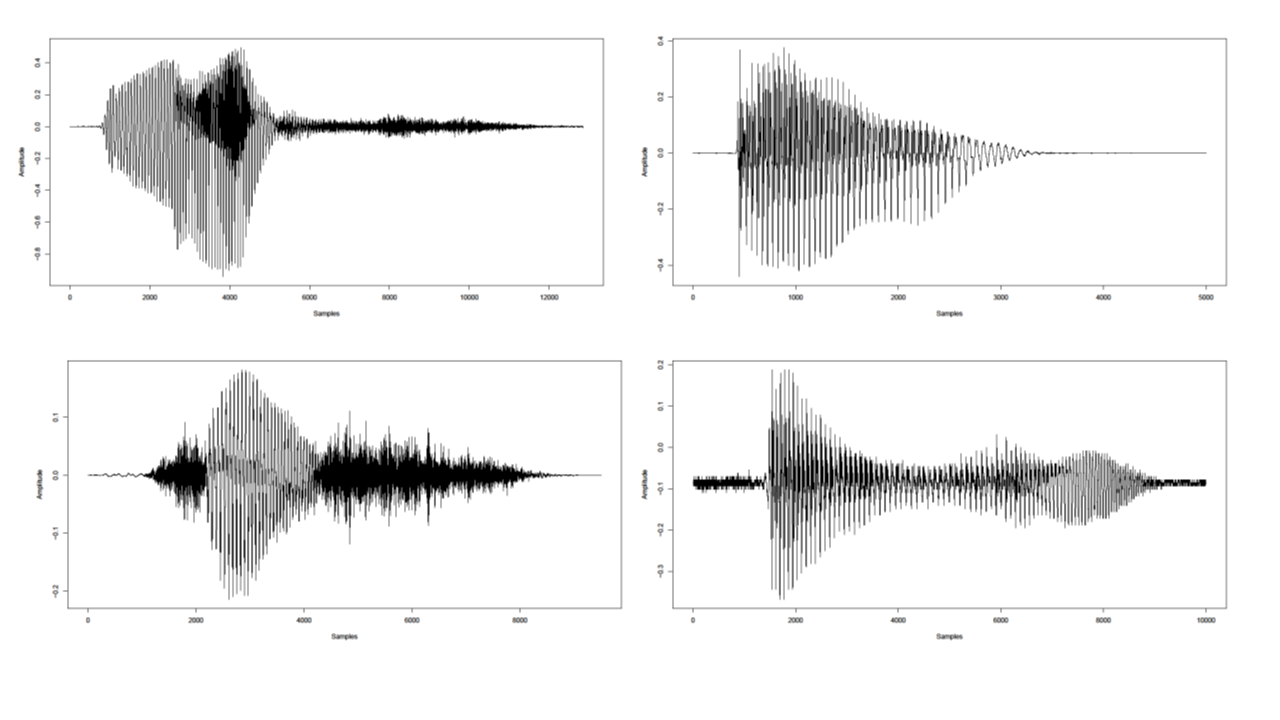
\includegraphics[width=15cm]{images/Interpolation/4 plot image.png}
    \caption{4 sample raw wave plots}
    \label{fig:4plot} 
\end{figure}

Notice the difference in length on the x-axis (the number of samples) between the four graphs. Since each of the original data has different length in time and has the same sampling rate of 1,000 Hz, the length of the data differs from one another. Thus, we have to interpolate these data prior to performing dimensional reduction.

In order to successfully implement the PCA method, we are going to apply linear interpolation on the data file. By interpolating each of the 219 acoustic signals, which were in various length, it would be compressed or lengthened to fit in the same length of 5000 data points. Each data point represents the amplitude of one millisecond of the signal, so each acoustic signals would be interpolated into a 5 second length signal with a sample rate of 1000 Hz.

The actual process of interpolation itself is simply processed by the R language built-in function \emph{approx}(), which takes in two vectors \emph{x, y}, each representing the coordinates of points to be interpolated, and an additional set of values \emph{xout}, which sets the values of points of where the interpolation would take place. The function would return two lists \emph{x, y} which represents the interpolated coordinates \cite{Approx}.

Prior to interpolation we create an empty matrix \emph{itpData} with 5,000 columns, where we would append each interpolated acoustic signals (which would be produced in vector type objects.)

For the interpolation, we create a \emph{for}() loop with variable \emph{i} going from 1 to 219, which will be representing the index for the acoustic signals of original Romance language data file. We receive each of the 219 signal data as dataframe, reconstruct it into a vector as variable \emph{y}. we also create variable \emph{x}, which is a uniformly distributed vector of length 5,000, and \emph{xoutval}, which is a uniformly distributed vector of length 5,000 from 1 to the original length of the acoustic signal. 

We then use the function \emph{approx}() with variables \emph{x, y, xoutval} and store the produced result in an object \emph{templist}. We convert the second element of obejct \emph{templist}, which is the \emph{y} component of the interpolated data, into a vector by using the built-in function \emph{unlist}(), and append it to the matrix \emph{itpData} with the built-in function \emph{rbind}().

After the \emph{for}() loop iteration we now have a matrix \emph{itpData} of 220 rows and 5000 columns (1 additional row with all 0 values, which existed as a dummy row as we initiated the matrix), where each row, except the first row, is comprised of interpolated data. We convert it into a dataframe with built-in function \emph{data.frame}() into object \emph{finalDF}, remove the first row, and finally have a dataframe \emph{finalDF} with 219 rows and 5000 columns, where each row represents the interpolated acoustic signal from the original Romance language acoustic signals.

With the 219 interpolated data we can again produce wave plots. The following figures are several examples of the wave plots.

\begin{figure}[H]
    \centering
    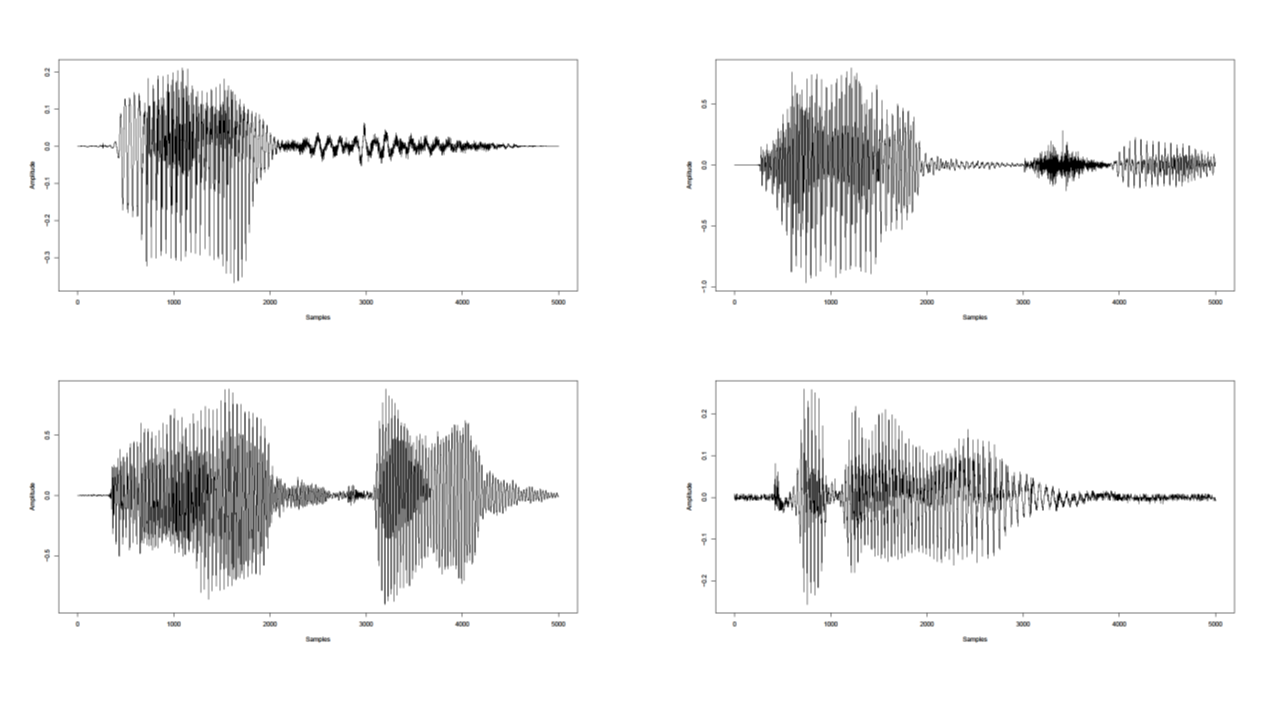
\includegraphics[width=15cm]{images/Interpolation/4 plot image (Inter).png}
    \caption{4 sample interpolated wave plots}
    \label{fig:4plotinter} 
\end{figure}

Notice that the length on the x-axis (the number of samples) of the four graphs are now fixed with 5,000 samples, as we have gone through the interpolation process. As the 219 data are aligned in same length, now the data is ready for dimensional reduction and further processing.


\newpage
\subsection{Spectrogram}


A spectrogram is a visual representation of the spectrum of frequencies of a signal as it varies over time. In other words, it shows how the energy of a signal is distributed across different frequencies at different points in time. Spectrograms are commonly used in signal processing and analysis, especially in fields like audio processing, speech recognition, and music analysis.

The basic idea behind a spectrogram is to take a signal, such as an audio recording, and divide it into short segments, typically ranging from a few milliseconds to a few seconds in length. For each segment, the spectrum of frequencies is computed using a mathematical technique called the Fourier transformation. The resulting spectrum is then displayed as a two-dimensional image, with time on the x-axis and frequency on the y-axis. The brightness or color of each pixel in the image represents the magnitude or energy of the corresponding frequency component.

By examining a spectrogram, it is possible to identify specific features of a signal that might not be apparent from the raw waveform. For example, in an audio signal, the spectrogram can reveal the presence of different harmonics and overtones, as well as variations in the amplitude and frequency content of the signal over time. Spectrograms can also be used to extract useful features for classification and recognition tasks, such as identifying different types of sounds or speech patterns.

Here is an example of a spectrogram. It is created from a sample audio file with duration of 33.5 seconds and sample rate of 8000 Hz. We read the \emph{.wav} audio file into a wave file in R with the \emph{readwave}() function in the \emph{tuneR} package. We can first plot the wave form of the file for future comparison with the spectrogram.

\begin{figure}[H]
    \centering
    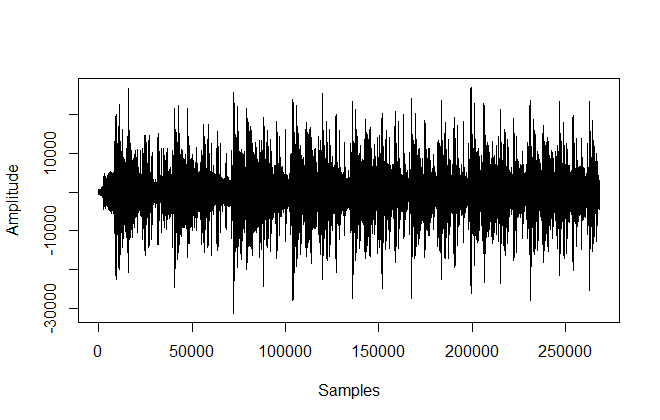
\includegraphics[width=12cm]{images/Spectrum/SampleWave.png}
    \caption{Wave form of the sample audio file}
    \label{fig:samplewave} 
\end{figure}

In order to construct a spectrogram we need to set some variable inputs. First, we shift the wave file by subtracting the mean of the signal in order to remove the DC offset. Then we set number of points to use, the window size, and the overlap. Then we can create a spectrogram with the built-in function \emph{specgram}() from the library \emph{signal}. 

The produced result \emph{spec} is a list-type data with three elements \emph{S, f, t}. Elements \emph{f} and \emph{t} are double-type objects that each represent the window size and number of points used. The element \emph{S} is a complex-type object which is the total data of the Spectrogram in a single row, having the multiplied value of \emph{f} and \emph{t} as its length.

We then go through several process on the element \emph{S} before creating a Spectrogram. We discard the phase information of \emph{S} and convert to a double-type object with function "\emph{abs}(), normalize it by dividing with the maximum amplitude \emph{max}(), and convert into dB unit by applying logarithm and multiplying by 10 unit \emph{10*log10}(). 

Now we can plot a spectrogram from the processed objects by using the built-in function \emph{imagep}() from the library \emph{oce}. We use \emph{t, f, S} as the \emph{x, y, z} component for the function \emph{imagep}() and can have the following figure as the resulting spetrogram.

\begin{figure}[H]
    \centering
    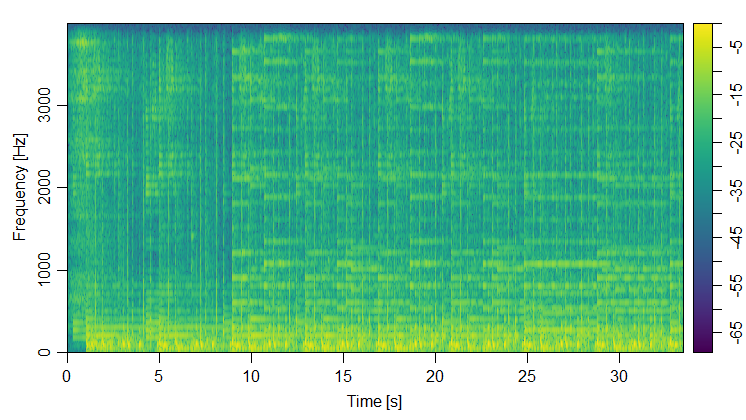
\includegraphics[width=12cm]{images/Spectrum/Spectrum (Processed).png}
    \caption{Spectrogram of the sample audio file}
    \label{fig:samplespectogram} 
\end{figure}

As we can see from the figure, Spectrograms are gnenrally a three-dimensional data set, with the third dimension displayed as colors. Time flows from left to right, which is from oldest to youngest, along the horizontal axis. The vertical axis denotes the frequency of the data, which can also be interpreted as pitch, with the lowest frequencies at the bottom and the highest frequencies at the top. The amplitude, which is also interpreted as loudness, of a particular frequency at a particular time is represented by the third dimension, color, with dark blues corresponding to low amplitudes and brighter colors up through red corresponding to progressively stronger amplitudes.

We can apply the same method of code to the interpolated dataframe of 219 acoustic signals to produce the spectrogram. We first create an empty matrix \emph{specData} with 19,456 columns (the length of the spectrogram of a single acoustic signal)  . We set the number of points to use as \emph{nfft} = 1024, widnow size as \emph{window} = 256, the overlap as \emph{overlap} = 128. Since the acoustic signals from the interpolated dataframe have 5,000 elements each, the duration and the sample rate can be set as \emph{dur} = 5 and \emph{fs} = 1,000 each.  

Now, similar to the case of interpolation, we create a \emph{for}() loop with variable \emph{i} going from 1 to 219, which will be representing the index for acoustic signals of the interpolated dataframe. We take an unlisted form of i-th row from the dataframe and store it in object \emph{snd} with the code \emph{unlist}(\emph{finalDF}[i, ]). To remove the DC offset we subtract each of 5,000 values in snd by its mean \emph{mean}(\emph{snd}). The following figure is the wave form image created from the first row of dataframe.

\begin{figure}[H]
    \centering
    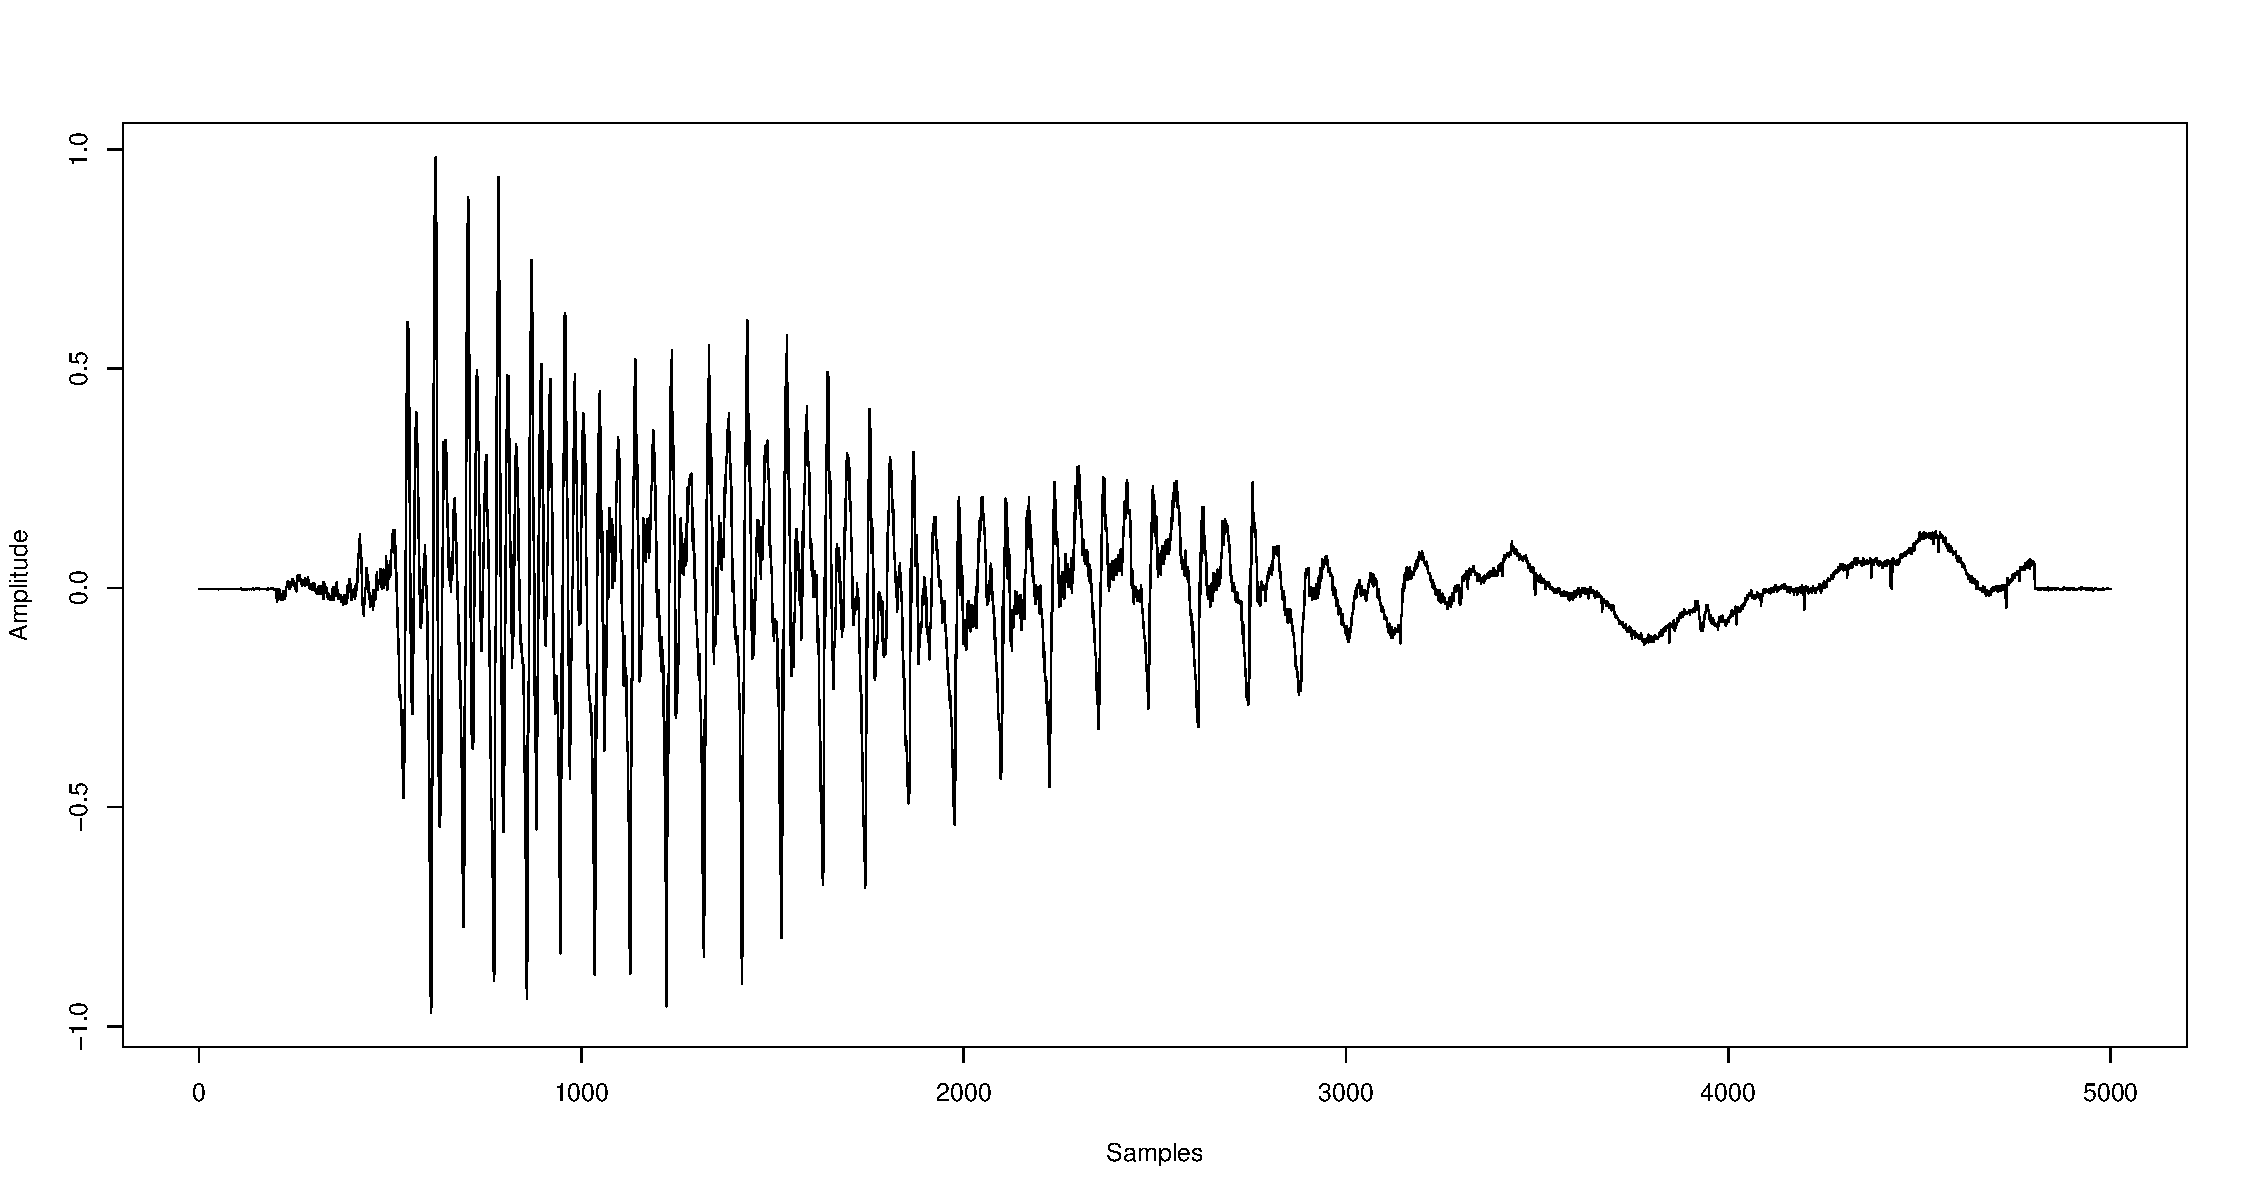
\includegraphics[width=12cm]{images/Spectrum/1RowWave.pdf}
    \caption{Wave form of the first Row of Dataframe}
    \label{fig:1RowWave} 
\end{figure}

Next, we put in the input variables \emph{snd, nfft, fs, window, overlap} into the function \emph{specgram}() and store the produced result in object \emph{spec}. We use the \emph{S} element from \emph{spec}, discard the phase information of \emph{S} with \emph{abs}(), convert to a double-type object with function "\emph{abs}(), normalize it by dividing with the maximum amplitude \emph{max}(), and convert into dB unit by applying logarithm and multiplying by 10 unit \emph{10*log10}().

Now we can plot the spectrogram by using \emph{imagep}() function and having its inputs as \emph{t, f, S} each representing the \emph{x, y, z} component. The following figure is the spectrogram image created from the first row of dataframe.

\begin{figure}[H]
    \centering
    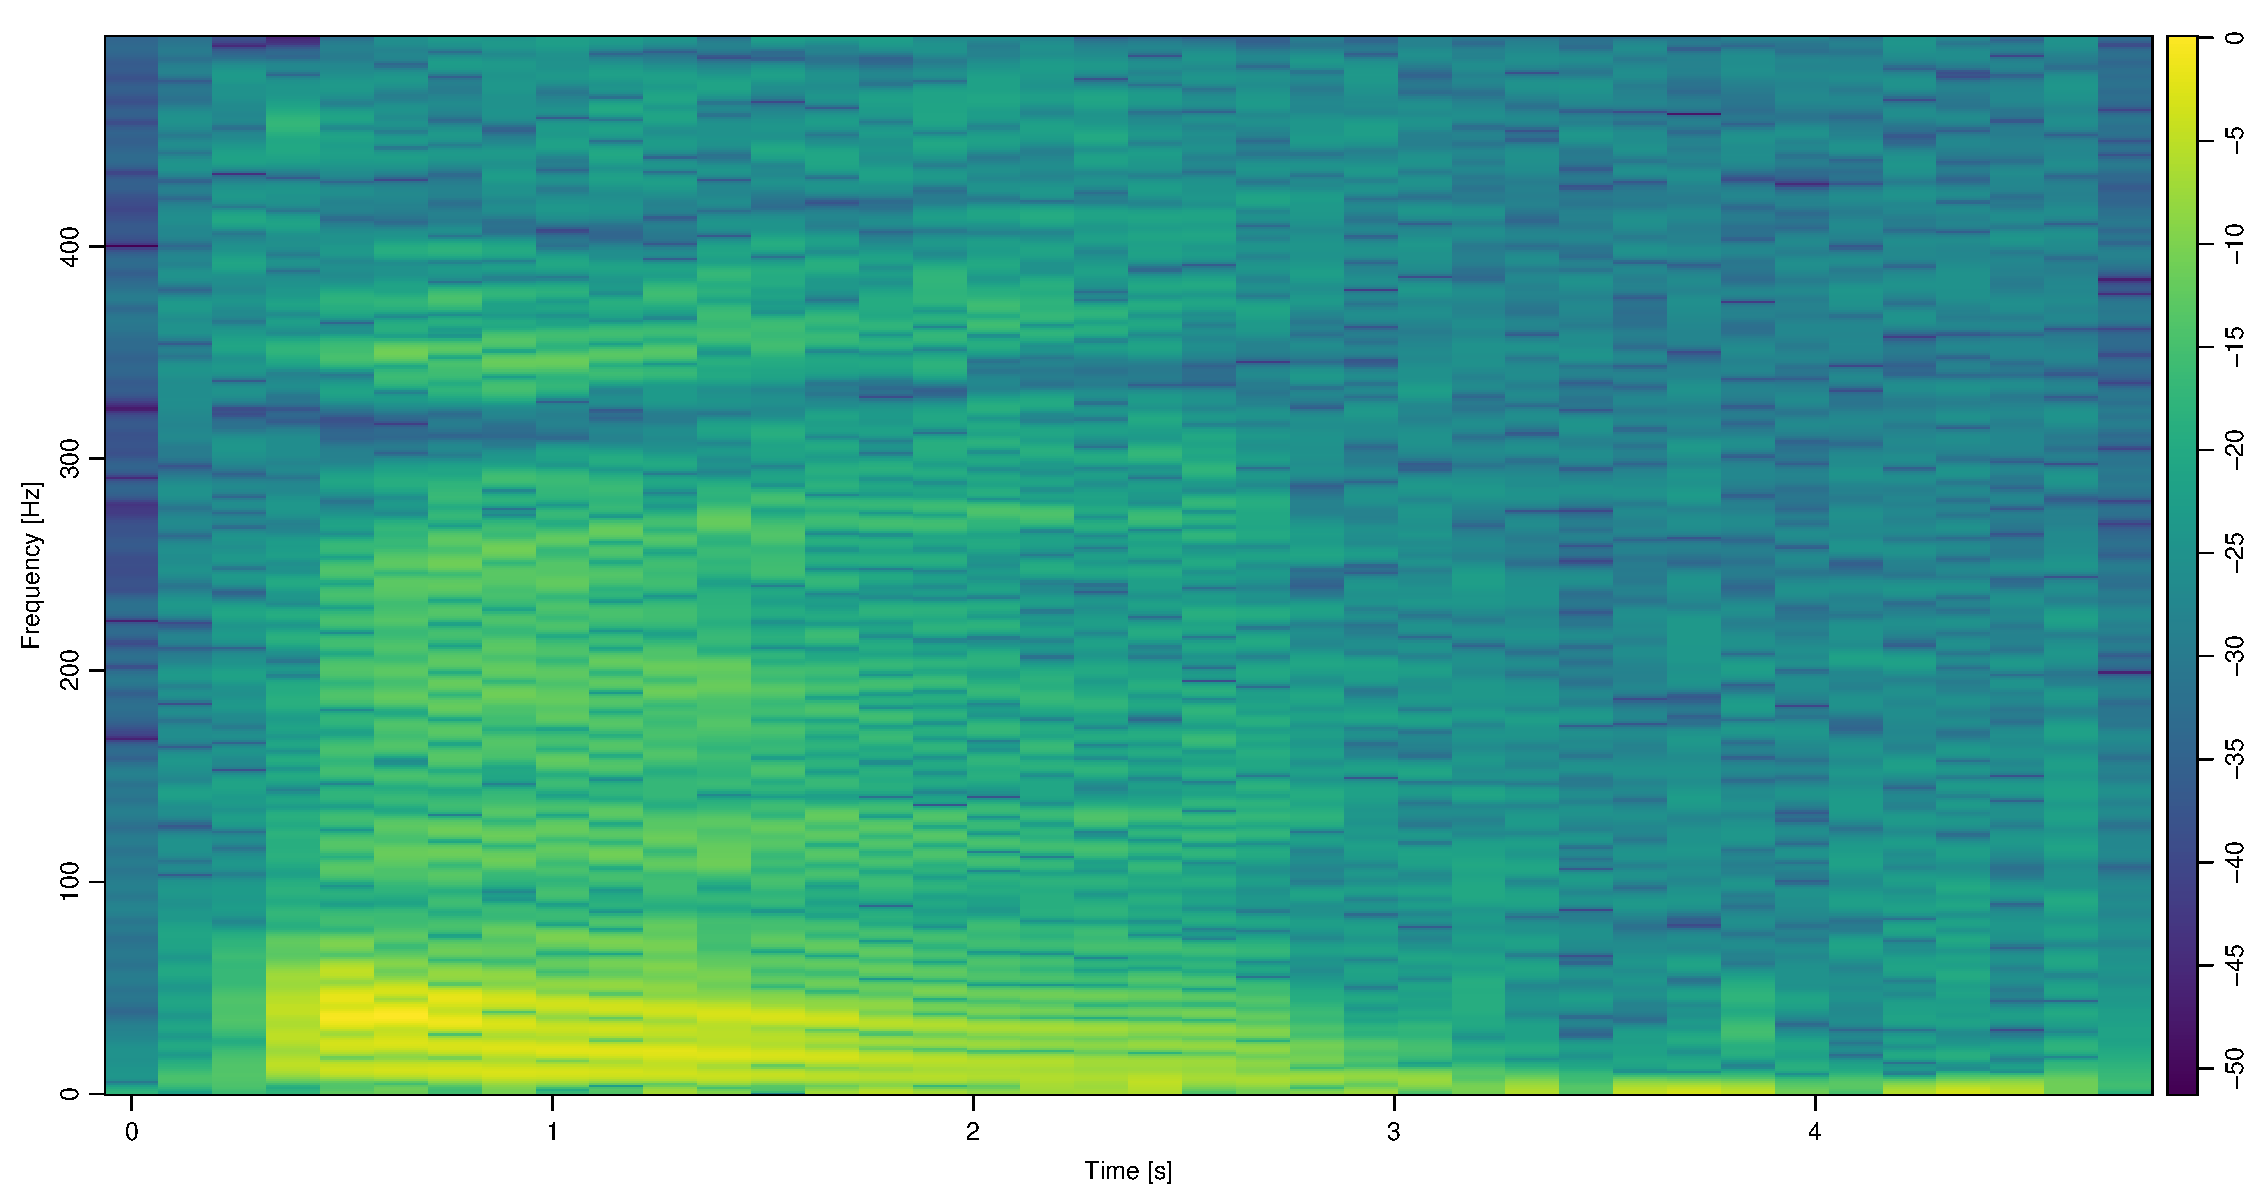
\includegraphics[width=12cm]{images/Spectrum/1Row Spec.pdf}
    \caption{Spectrogram of the first Row of Dataframe}
    \label{fig:1RowSpec} 
\end{figure}

Notice the difference in resolution compared to the example spectrogram from a sample audio file. The sample file had 33.5 seconds of duration and 8,000 Hz frequency, resulting in 33.5 * 4,000 size spectrogram (the frequency is halved as we discarded the phase information by normalizing \emph{S}), while this spectrogram has 5*500 size. The difference in the color brightness and pattern, which is the \emph{S} component from the spectrogram, shows the difference in the variance of amplitude of the two.

Finally, we can store the \emph{S} component as a row in our matrix \emph{specData} via the function \emph{rbind}().

After the \emph{for}() loop iteration we now have a matrix \emph{specData} of 220 rows and 19456 columns. We convert it into a dataframe with \emph{data.frame}() and store it into object \emph{finalSpec}, remove the first row, and finally we have a dataframe \emph{finalSpec} with 219 rows and 19456 columns, where each row correctly represents the spectrum of the original interpolated data.


\newpage
\section{Application of Principal Component Analysis on Acoustic Signals via R}


With the processed data, original and spectrum, we can proceed with the application of PCA. The actual application of PCA via R is simply performed by the built-in function \emph{prcomp}() \cite{Chazal}.


\subsection{PCA on original dataframe}


By inserting original data frame as the input variable on the function \emph{prcomp}(), we generate a PCA processed data and store it in the variable \emph{my-pca}. 

The resulting object \emph{my-pca} is a large prcomp-type data with 5 elements: \emph{sdev, rotation, center, scale, x}. The \emph{sdev} holds the standard deviation for each 219 principal components, and the other four elements holds 219 data of the relevant information for each 219 principal components. Therefore, \emph{my-pca} stores 219 elements, each representing a principal component, which are each 219 length, thus comprising a 219 x 219 dataframe.

The 219 principal components processed in \emph{my-pca} are ordered from highest variance to the lowest, meaning the first few principal components are the most important data to look into. We would select the first three principal components, naming each of them \emph{PC1, PC2, PC3}, and construct three different biplots by putting x and y axis with the combinations of these three principal components.

\begin{figure}[H]
    \centering
    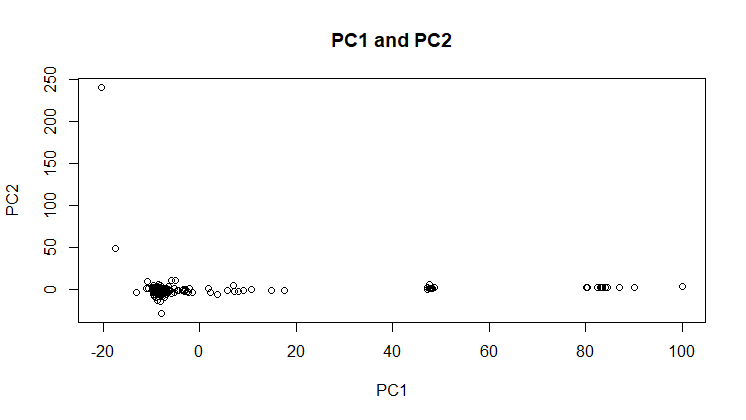
\includegraphics[width=12cm]{images/PCA/PC1 and PC2.png}   
    \caption{Biplot of PC1 and PC2}
    \label{fig:PCA12biplot} 
\end{figure}

\begin{figure}[H]
    \centering
    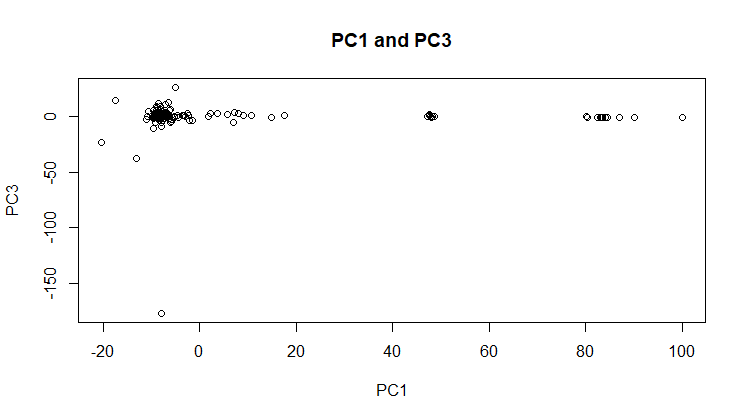
\includegraphics[width=12cm]{images/PCA/PC1 and PC3.png}
    \caption{Biplot of PC1 and PC3}
    \label{fig:PCA13biplot} 
\end{figure}

\begin{figure}[H]
    \centering
    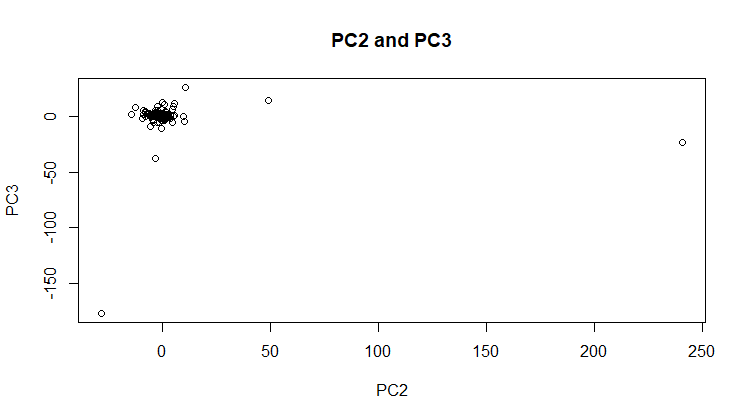
\includegraphics[width=12cm]{images/PCA/PC2 and PC3.png}
    \caption{Biplot of PC2 and PC3}
    \label{fig:PCA23biplotd} 
\end{figure}

We can analyze the nature of each principal components by observing the points on these biplots \cite{PCAbiplot}. The corresponding score of each points along the x and y axis is proportionate to the strength regarding the principal component of the axis. 

For instance, if we closely examine figure 7 and figure 8 we notice that there are several points heading to the far right along the x-axis, which is PC1. This tells that these points have strong scores on the PC1 component. 

The cluster of the points also describes the relative character and the general structure of the principal components. If we observe figure 1, we can confirm that there exists a central cluster near value -10 for PC1 and value 0 for PC2. We can also confirm that there lies a single point on the far up-left corner. This single point can be interpreted as an outlier for the PC2 component, as the 219 points for PC2 are mostly distributed near value 0 and forms a strong cluster group around the are.

The same attribute can be confirmed from PC3 component as well by observing figure 2. Most of the points are distributed near the value of 0 and forms a strong cluster group near the are, and there lies a single outlier on the bottom-left corner of the plot. By observing figure 9, where the cluster group is most heavily centered near the value 0 for both PC2 and PC3, we can observe that PC1 forms higher variance compared to PC2 and PC3

Now we should compute the variance in order to calculate the number of principal components to use and to neglect in order to reduce the dimension of the data. We can square the standard deviation given from the element \emph{sdev} from \emph{my-pca} to calculate the variance of each 217 principal components.

Then we calculate the proportion of variance of each principal components by dividing each variance with the total sum of 219 variances. We can now plot a scree plot with x-axis being the principal components and y-axis being the proportion of variance of the principal components.

\begin{figure}[H]
    \centering
    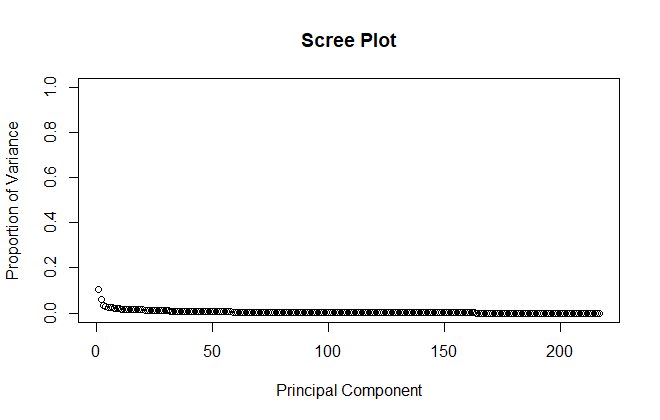
\includegraphics[width=12cm]{images/PCA/Scree Plot.png}
    \caption{Scree Plot}
    \label{fig:screeplot} 
\end{figure}

We can also construct a cumulative scree plot, which has y-axis as the cumulative proportion of variance instead.

\begin{figure}[H]
    \centering
    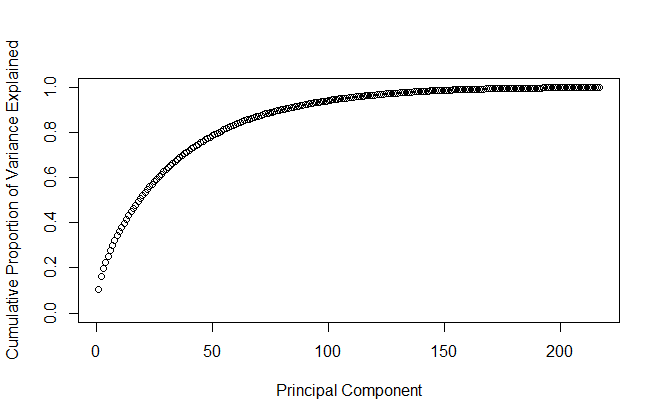
\includegraphics[width=12cm]{images/PCA/Cumulative Scree Plot.png}
    \caption{Cumulative Scree Plot}
    \label{fig:cumscreeplot} 
\end{figure}

We can notice from the plot that the first three principal components contributes to roughly 20 percent of the total variance and the first 12 principal components contributes to roughly 40 percent of the total variance.

We can now compute the number of principal components (chosen by the given order since it is already arranged by variance) to use and to neglect, depending on the percentage of the variance. In order to take account of 80 percent of the variance we get a calculated result of 53 (roughly 75.5 percent reduction in dimension). In order for 90 percent and 95 percent we get a calculated result of 79 (roughly 64 percent reduction in dimension) and 105 (roughly 52 percent reduction in dimension) each. 

In conclusion the overall result of the principal component analysis applied on interpolated 219 acoustic signal data resulted on generating 219 principal components. By calculating the proportion of variance, we concluded with a calculation that roughly 75.5, 64, and 52 percent of dimension out of 219 dimensions can be reduced in order to consider 80, 90, 95 percent of the total variance. 


\newpage
\subsection{PCA on Spectrum}


We can apply PCA on the spectrum dataframe \emph{finalSpec} through similar process as we did in the above section. The key difference between the two dataframes is in the length of each variables: the number of columns. While the original interpolated dataframe has 5,000 columns, the spectrum dataframe has 19,456 columns. The difference, however, does not heavily affect in the general results as the dimension of the principal components remains the same since as each of the 219 rows of two dataframes relates to the same acoustic signals.

We insert \emph{finalSpec} into function \emph{prcomp}() and store the result in object \emph{my-pca}. 

The resulting data \emph{my-pca} consists with 5 elements: \emph{sdev, rotation, center, scale, x}. The \emph{sdev} holds the standard deviation for each 219 principal components of the spectrum dataframe, and the other four elements holds 219 data of the relevant information for each 219 principal components. 

Now we construct the biplots of the firs three principal components.

\begin{figure}[H]
    \centering
    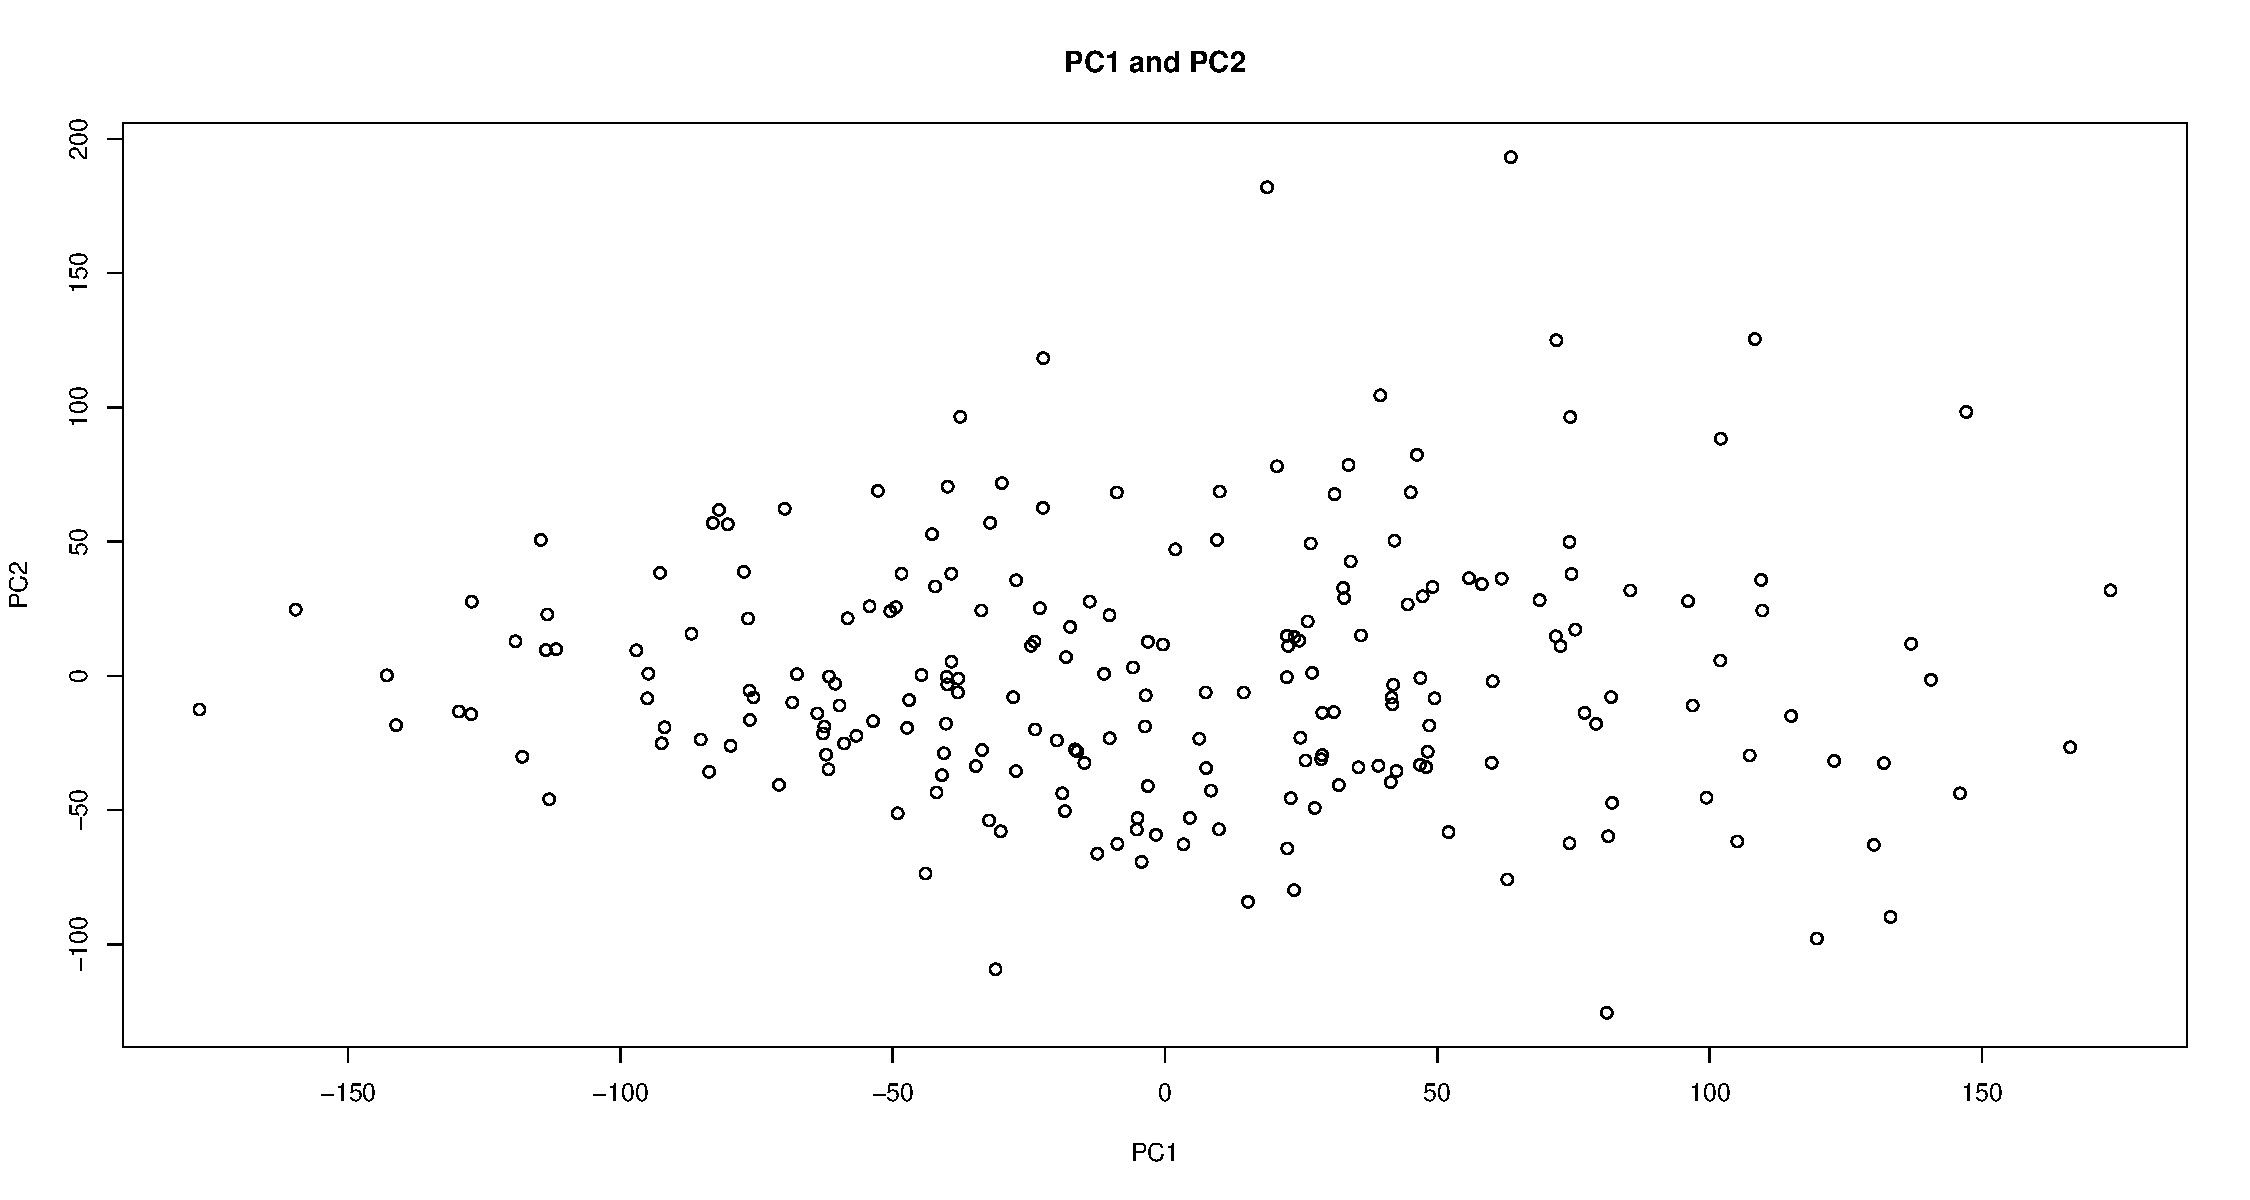
\includegraphics[width=12cm]{images/PCA (Spec)/PC1 and PC2.pdf}  
    \caption{Biplot of Spectrum's PC1 and PC2}
    \label{fig:PCASpec12biplot} 
\end{figure}

\begin{figure}[H]
    \centering
    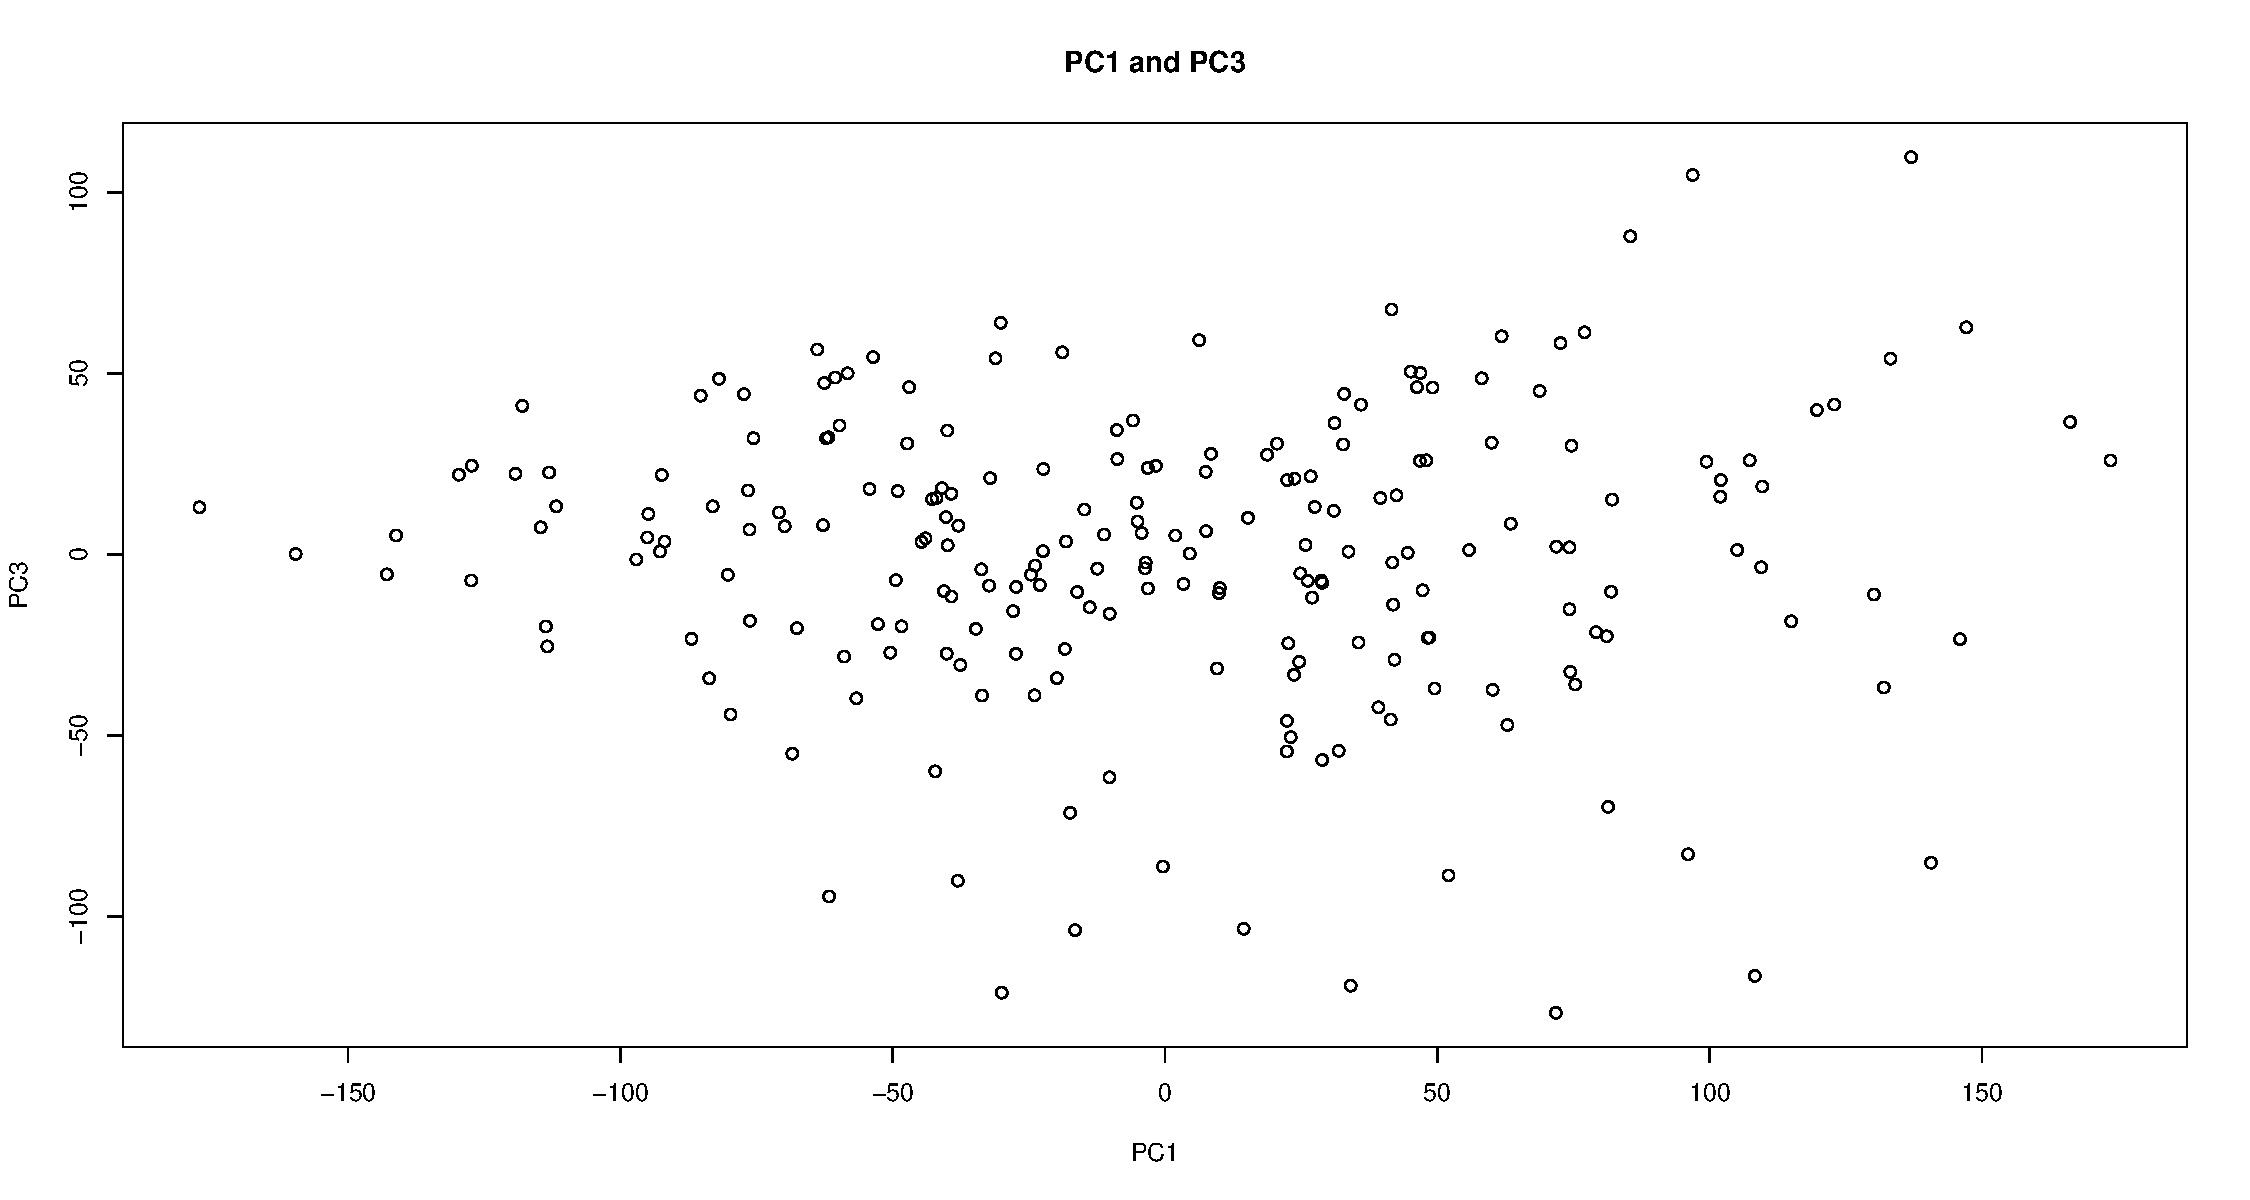
\includegraphics[width=12cm]{images/PCA (Spec)/PC1 and PC3.pdf}
    \caption{Biplot of Spectrum's PC1 and PC3}
    \label{fig:PCASpec13biplot} 
\end{figure}

\begin{figure}[H]
    \centering
    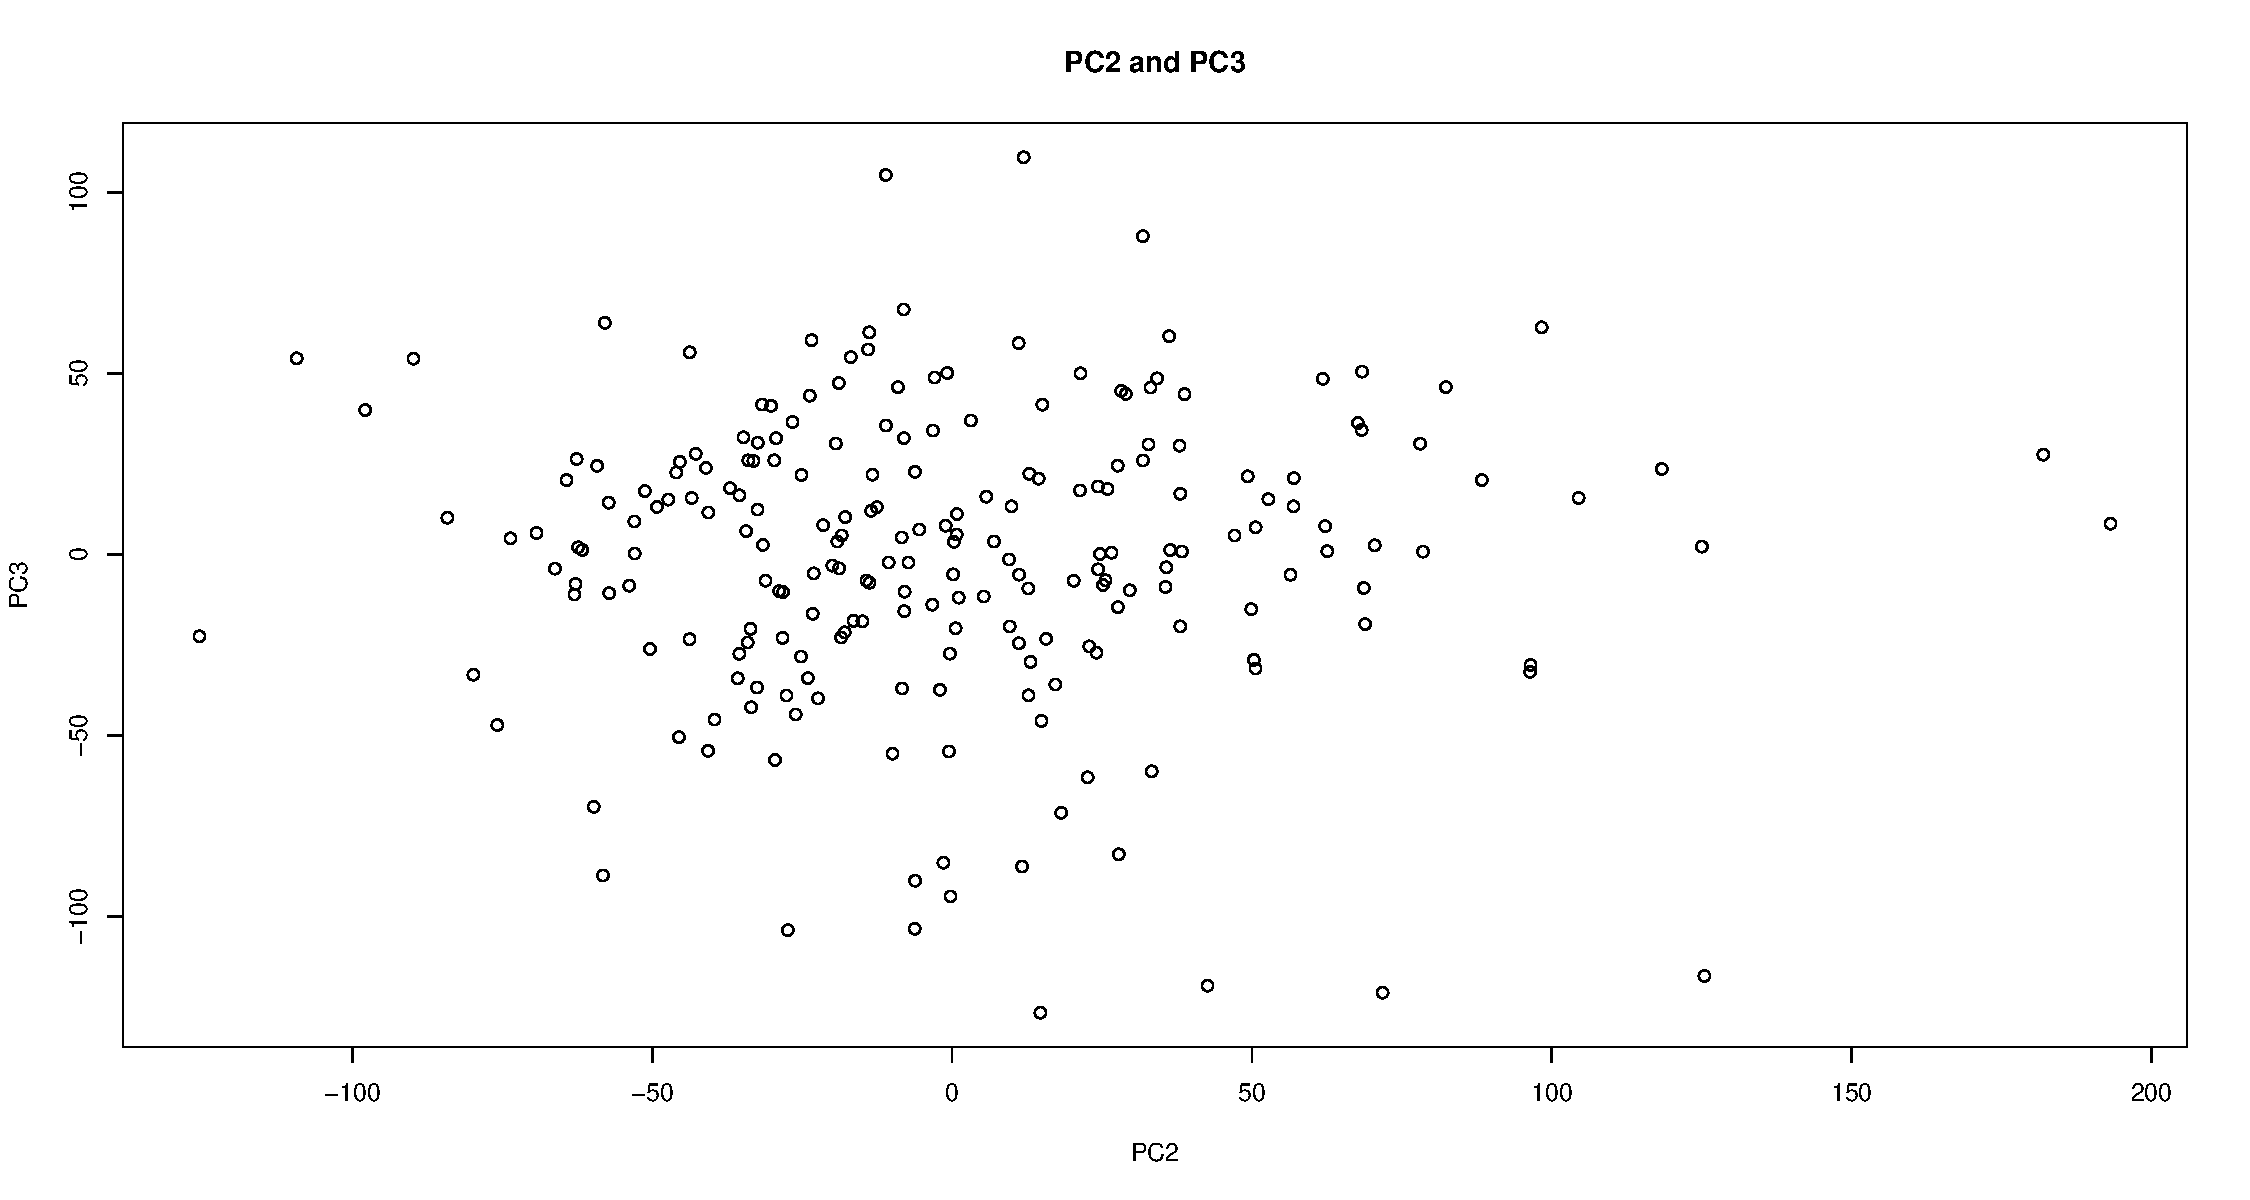
\includegraphics[width=12cm]{images/PCA (Spec)/PC2 and PC3.pdf}
    \caption{Biplot of Spectrum's PC2 and PC3}
    \label{fig:PCASpec23biplotd} 
\end{figure}

We can see that there is a much wider spread on the biplots between the three principal components compared to the case of original dataframe. There seems to be no obvious observable cluster groups among the three biplots, which can be interpreted that the three principal components are all widely spread and has moderate variance.
This may be due to the difference in the length of each spectrum, since it almost has 4 times difference from the original dataframe.

Now we should calculate and compare the variance for each 219 principal components. Then we calculate the proportion of variance of each principal components and produce a scree plot.

\begin{figure}[H]
    \centering
    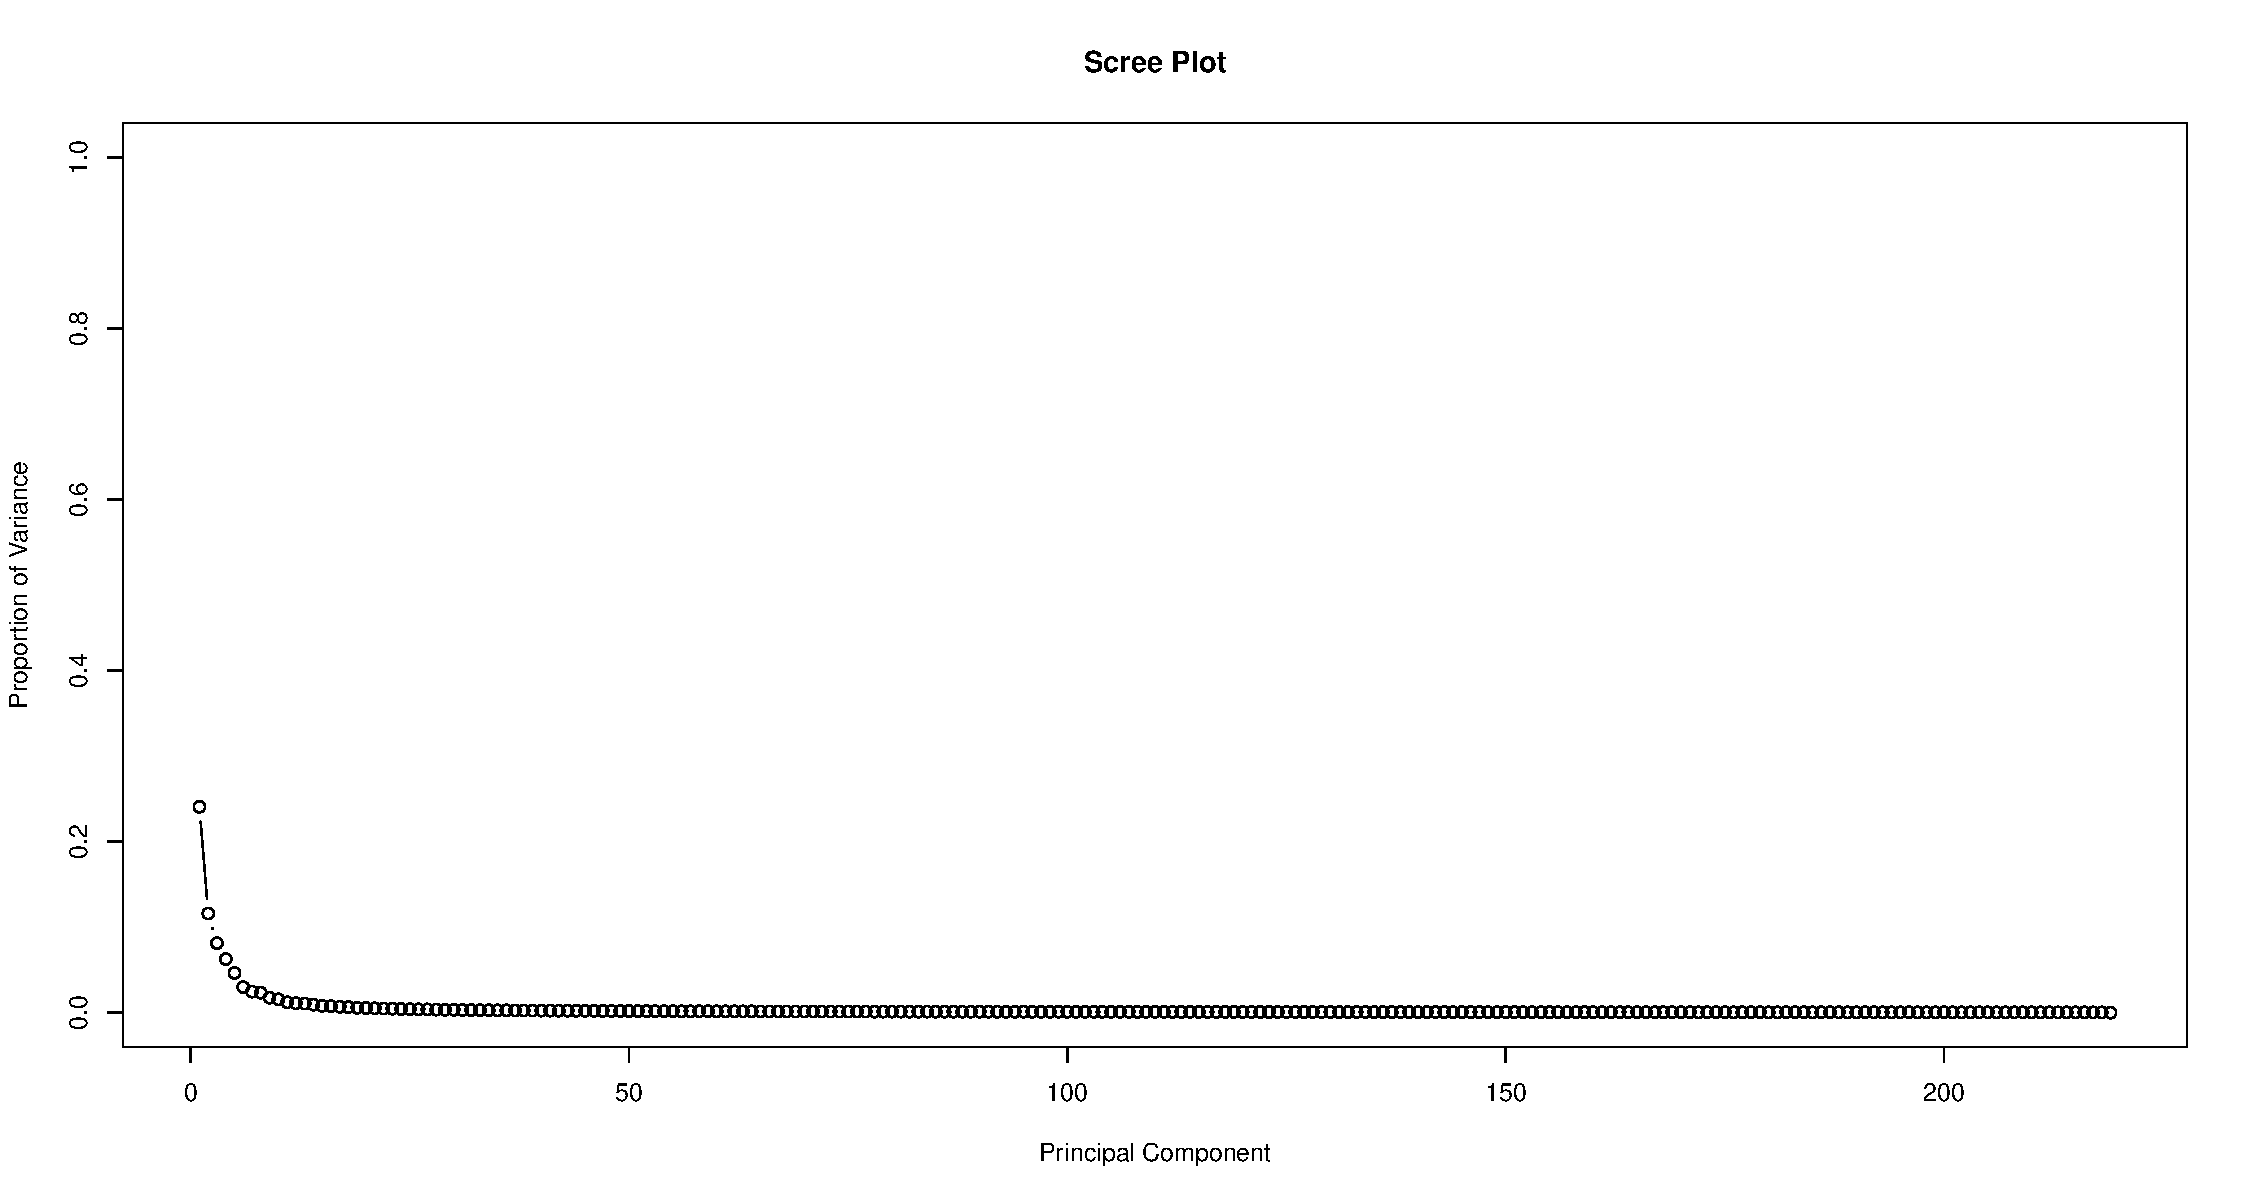
\includegraphics[width=12cm]{images/PCA (Spec)/Scree Plot.pdf}
    \caption{Spectrum's Scree Plot}
    \label{fig:Spec screeplot} 
\end{figure}

We can also construct a cumulative scree plot, which has y-axis as the cumulative proportion of variance instead.

\begin{figure}[H]
    \centering
    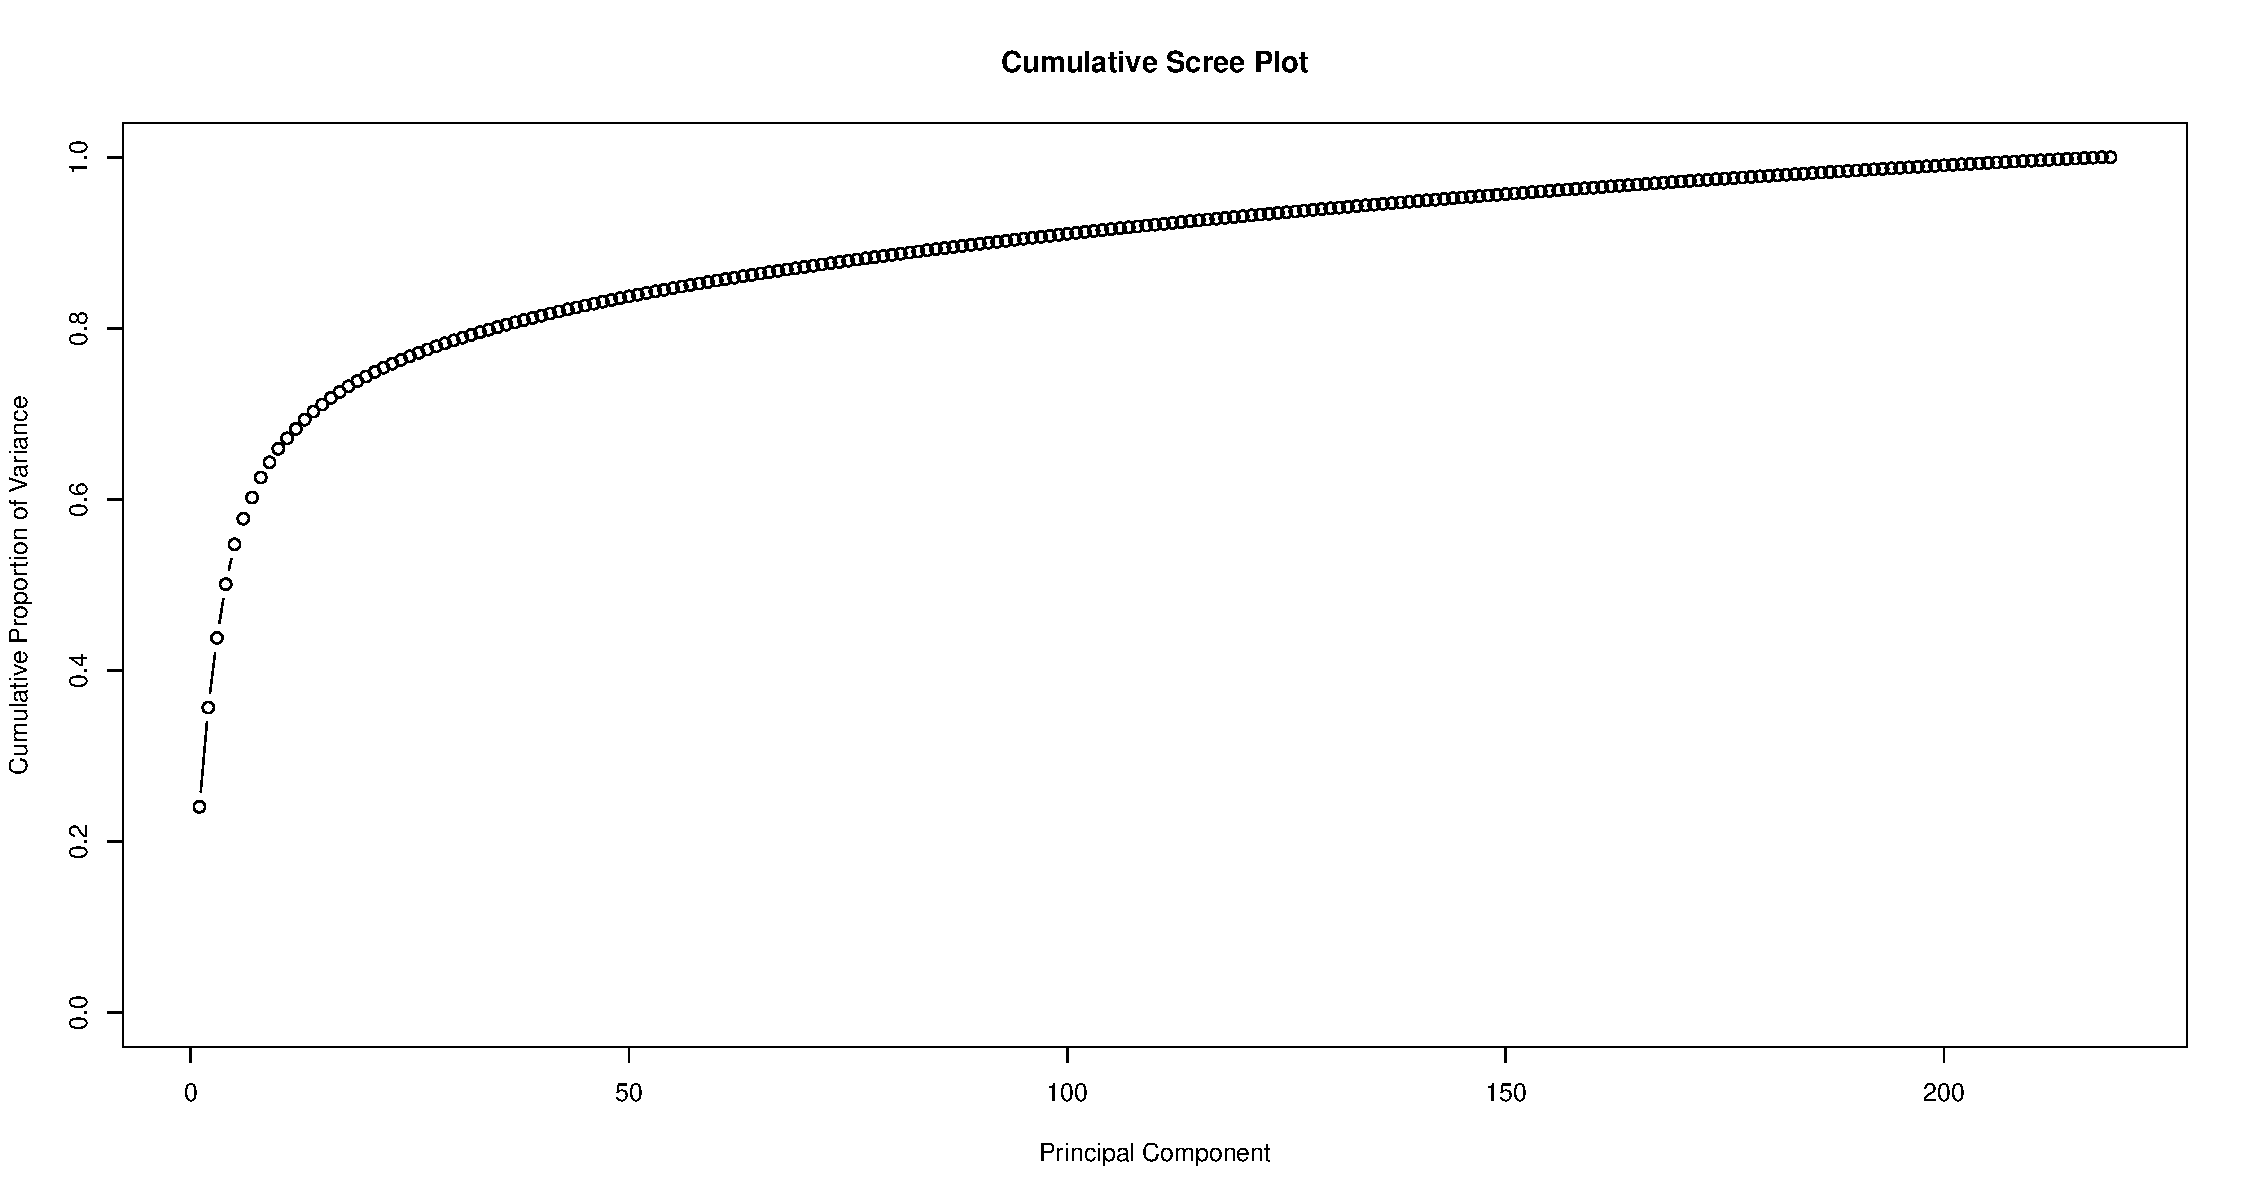
\includegraphics[width=12cm]{images/PCA (Spec)/Cumulative Scree Plot.pdf}
    \caption{Spectrum's Cumulative Scree Plot}
    \label{fig:Spec cumscreeplot} 
\end{figure}

We can notice from the plot that the first three principal components contributes to roughly 20 percent of the total variance and the first 12 principal components contributes to roughly 40 percent of the total variance.

We can notice that the first principal component contributes significantly higher in variance than the rest, up to roughly 21 percent of the total variance. Although the first principal component has a significant difference in the variance than the others, the second and third principal component also contributes to a substantial amount of variance, which supports the observations from figure 12, 13, and 14. The first three principal components contributes to roughly 42 percent of the total variance and the first 7 principal components contributes to roughly 60 percent of the total variance.

Compared to the results from original dataframe, we can observe that the first few key principal components contributes to a much more significant amount of variance in the results from spectrum dataframe.

We can now compute the number of principal components to use and to neglect, depending on the percentage of the variance. In order to take account of 80 percent of the variance we get a calculated result of 35 (roughly 84 percent reduction in dimension). In order for 90 percent and 95 percent we get a calculated result of 92 (roughly 58 percent reduction in dimension) and 142 (roughly 35 percent reduction in dimension) each. 

In conclusion the overall result of the principal component analysis applied on spectrum of 219 acoustic signal data resulted on generating 219 principal components. By calculating the proportion of variance, we concluded with a calculation that roughly 84, 58, and 35 percent of dimension out of 219 dimensions can be reduced in order to consider 80 , 90, 95 percent of variance. 

Notice that for the 80 percent of variance, PCA on spectrum dataframe has a much more efficient outcome compared to original dataframe (roughly 8.5 percent more reduction). However, PCA on original dataframe becomes much more efficient for 90, 95, and further percent of variance (roughly 6 and 17 percent more reduction).


\newpage
\subsection{PCA on original dataframe separated by language}


Now we perform the PCA on original dataframe separated by the five romance langauges: Portuguese, Italian, Iberian Spanish, French, and American Spanish. First we divide the dataframe \emph{finalDF} into parts that corresponds to each languages (Portuguese, Italian, Iberian Spanish, French, and American Spanish) and save them in objects \emph{finalDFPO, finalDFIT, finalDFSI, finalDFFR, finalDFSA}. Index 1 to 25 of \emph{finalDF} consists of Portuguese, 27 to 75 on Italian, 76 to 113 on Iberian Spanish, 114 to 173 on French, and 174 to 219 on American Spanish. The length of the index is the dimension for each languages.

Now we perform PCA on the five dataframe objects \emph{finalDFPO, finalDFIT, finalDFSI, finalDFFR, finalDFSA}. 

The following figures are the biplots for first three principal components and the cumulative scree plot for the dataframe \emph{finalDFPO}.

\begin{figure}[H]
    \centering
    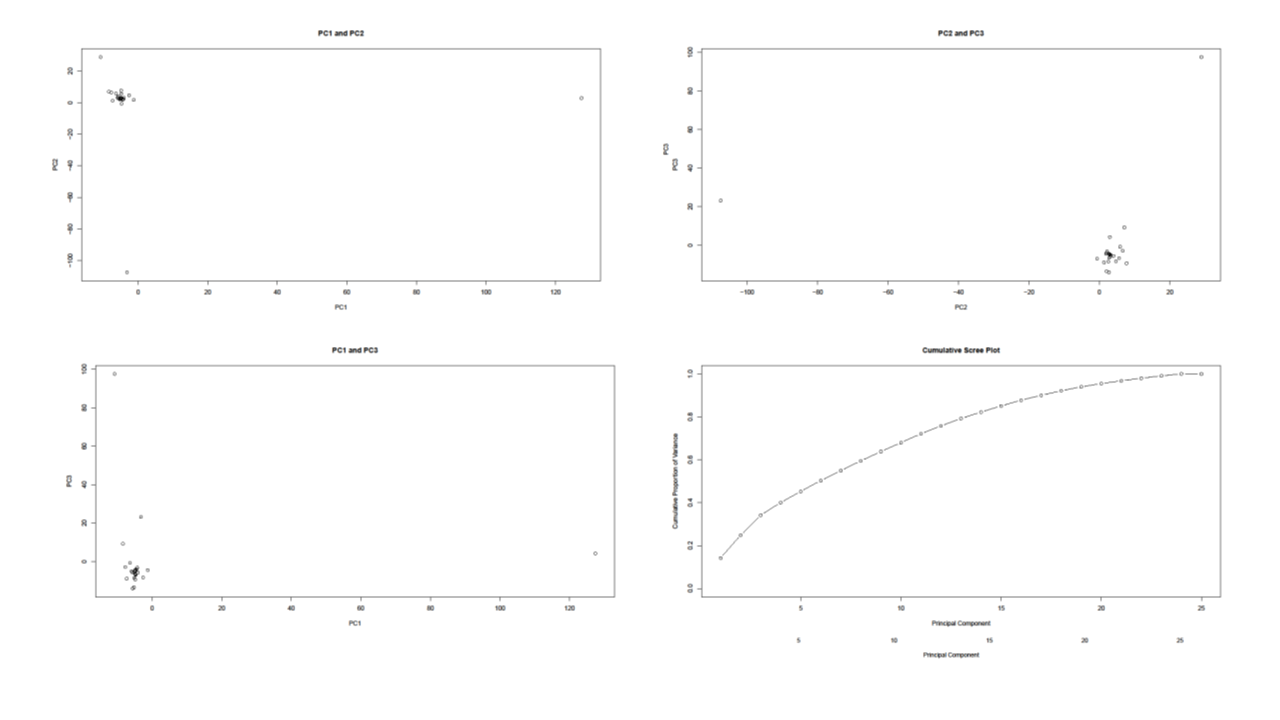
\includegraphics[width=15cm]{images/PCA/4plotPO.png}
    \caption{Biplot and Screeplot of Portuguese Dataframe}
    \label{fig:4plotPO} 
\end{figure}

We can observe that the three biplots all form a strongly gathered cluster group with negligible number of outliers.

Out of total 25 principal components, in order to take account of 80 percent of the variance we get a calculated result of 14 (roughly 44 percent reduction in dimension). In order for 90 percent and 95 percent we get a calculated result of 17 (roughly 32 percent reduction in dimension) and 20 (roughly 20 percent reduction in dimension) each. 

Notice that the three biplots of the first three principal components forms a highly gathered cluster.

The following figures are the biplots for first three principal components and the cumulative scree plot for the dataframe \emph{finalDFIT}.

\begin{figure}[H]
    \centering
    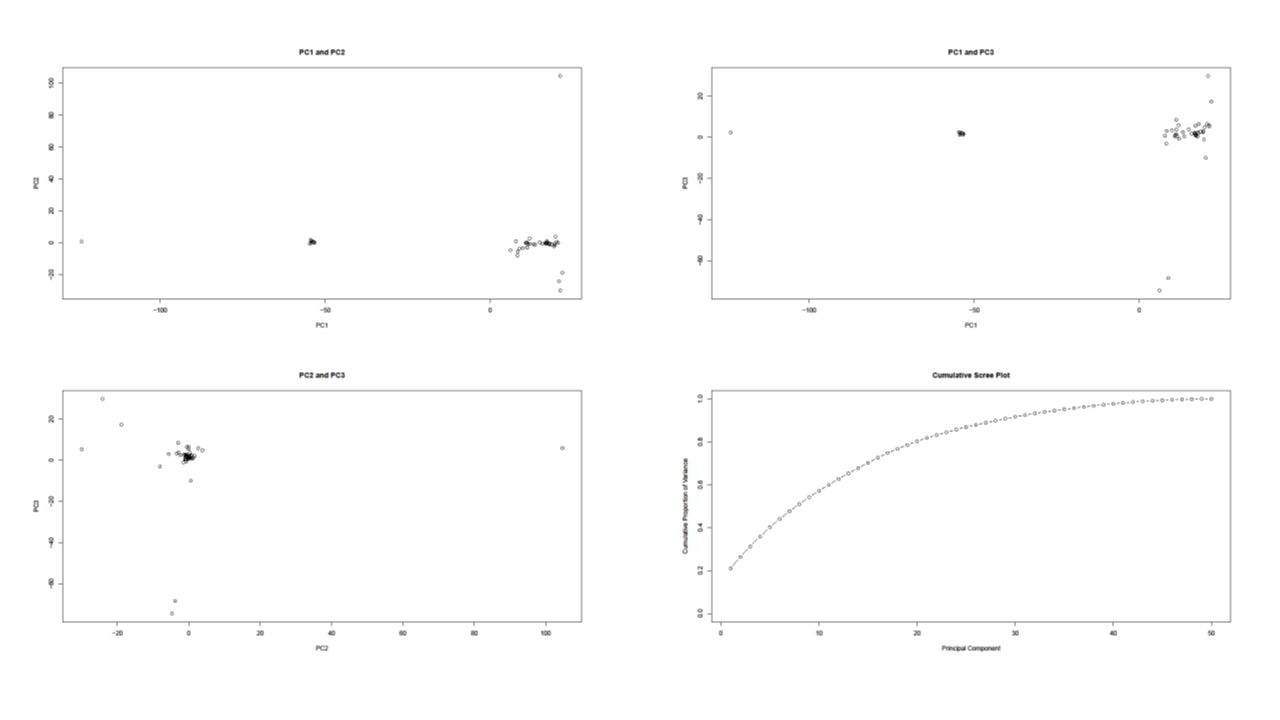
\includegraphics[width=15cm]{images/PCA/4plotIT.png}
    \caption{Biplot and Screeplot of Italian Dataframe}
    \label{fig:4plotIT} 
\end{figure}

We can observe that the three biplots all form a moderately gathered cluster group with some number of outliers, even forming a trivial cluster group on the top two figures.

Out of total 50 principal components, in order to take account of 80 percent of the variance we get a calculated result of 20 (roughly 60 percent reduction in dimension). In order for 90 percent and 95 percent we get a calculated result of 29 (roughly 42 percent reduction in dimension) and 35 (roughly 30 percent reduction in dimension) each. 

The following figures are the biplots for first three principal components and the cumulative scree plot for the dataframe \emph{finalDFSI}.

\begin{figure}[H]
    \centering
    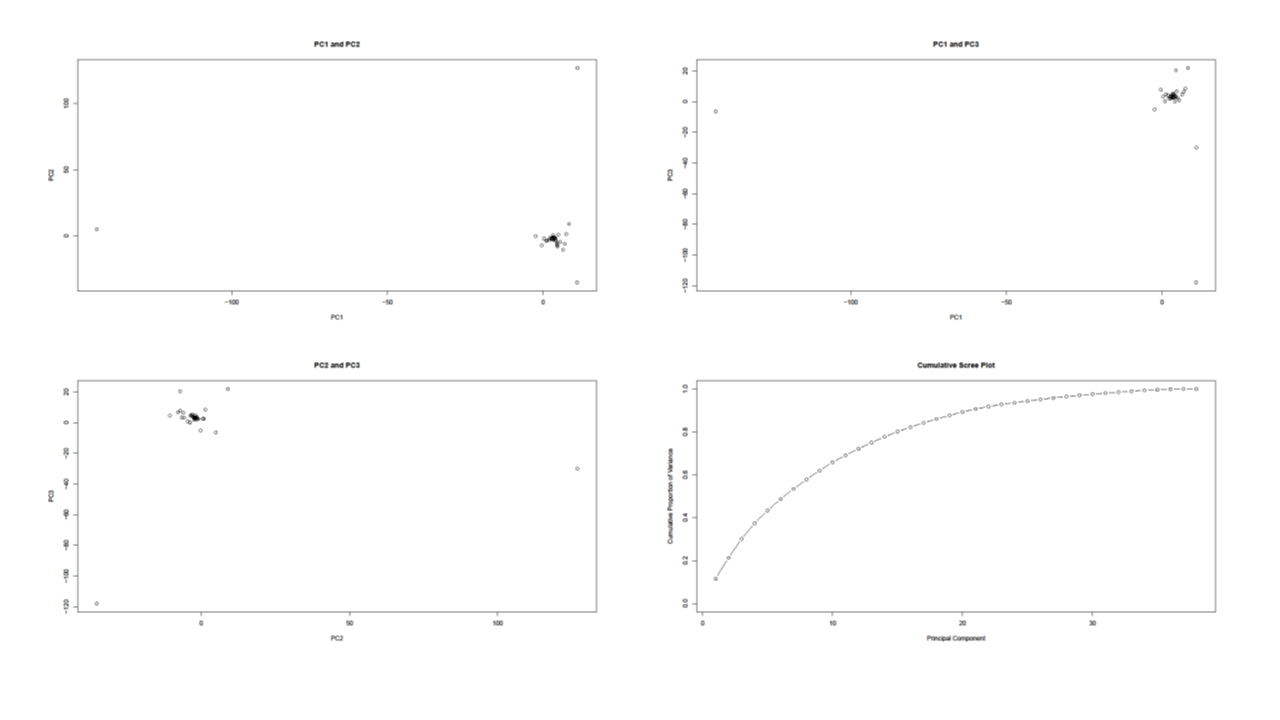
\includegraphics[width=15cm]{images/PCA/4plotSI.png}
    \caption{Biplot and Screeplot of Iberian Spanish Dataframe}
    \label{fig:4plotSI} 
\end{figure}

We can observe that the three biplots all form a strongly gathered cluster group with negligible number of outliers, similar to observation from the Portuguese dataframe.

Out of total 38 principal components, in order to take account of 80 percent of the variance we get a calculated result of 15 (roughly 60.5 percent reduction in dimension). In order for 90 percent and 95 percent we get a calculated result of 21 (roughly 45 percent reduction in dimension) and 26 (roughly 31.5 percent reduction in dimension) each. 

The following figures are the biplots for first three principal components and the cumulative scree plot for the dataframe \emph{finalDFFR}.

\begin{figure}[H]
    \centering
    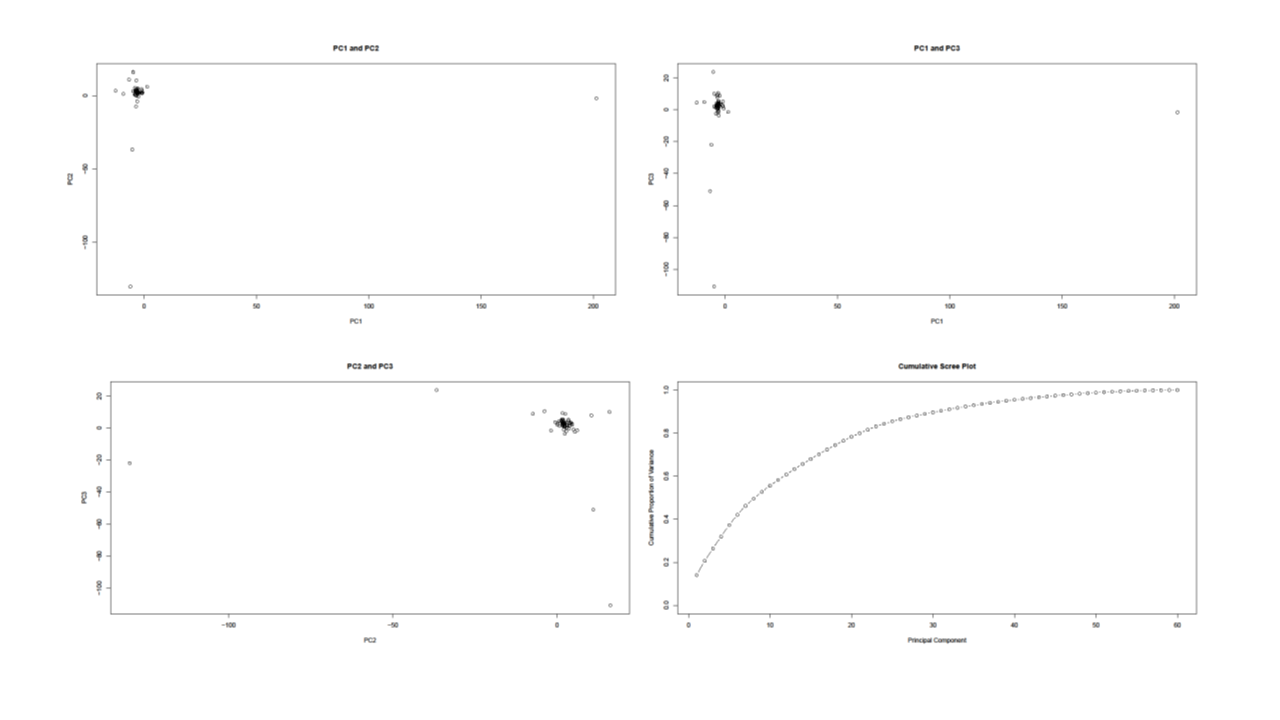
\includegraphics[width=15cm]{images/PCA/4plotFR.png}
    \caption{Biplot and Screeplot of French Dataframe}
    \label{fig:4plotFR} 
\end{figure}

We can observe that the three biplots all form a strongly gathered cluster group with few number of outliers, similar to observation from the Portuguese and Iberian Spanish dataframe.

Out of total 60 principal components, in order to take account of 80 percent of the variance we get a calculated result of 22 (roughly 63 percent reduction in dimension). In order for 90 percent and 95 percent we get a calculated result of 31 (roughly 48.5 percent reduction in dimension) and 39 (roughly 35 percent reduction in dimension) each. 

The following figures are the biplots for first three principal components and the cumulative scree plot for the dataframe \emph{finalDFSA}.

\begin{figure}[H]
    \centering
    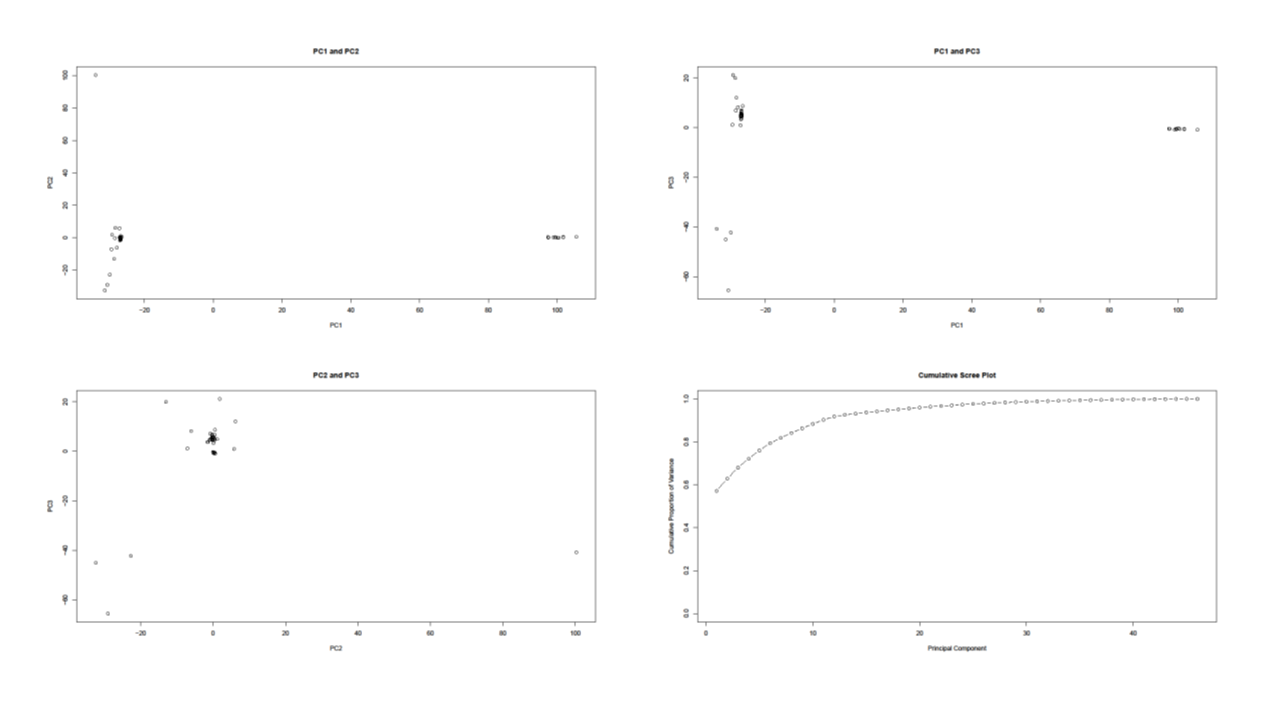
\includegraphics[width=15cm]{images/PCA/4plotSA.png}
    \caption{Biplot and Screeplot of American Spanish Dataframe}
    \label{fig:4plotSA} 
\end{figure}

We can observe that the three biplots does not form a strong and uniform cluster groups, and has the most spread and variance among the five language group dataframes.

Out of total 46 principal components, in order to take account of 80 percent of the variance we get a calculated result of 7 (roughly 85 percent reduction in dimension). In order for 90 percent and 95 percent we get a calculated result of 11 (roughly 76 percent reduction in dimension) and 18 (roughly 61 percent reduction in dimension) each. 

Notice the significantly high percent of reduction in dimension along all range of percent of variance. By observing the cumulative scatter plot, we can understand that it is due to substantially high contribution by the first principal component.
\newpage
\section{Application of Independent Component Analysis on Acoustic Signals via R}   


With the preprocessed data, we can proceed with the application of ICA. Note that among various algorithms for ICA, in this dissertation we focus on using the \emph{fastICA}. In R language we would use the function \emph{fastICA()} from the package \emph{fastICA}.

The code for processing ICA is much simpler than PCA; we consider the two main variables \emph{x} and \emph{n.comp} in the function \emph{fastICA}(). The variable \emph{x} holds multidimensional signal matrix (or dataframe), where each row represents observations (the signal data) and each column represents variables (sampling points). The variable \emph{n.comp} holds a numeric value, which is the number of components to be extracted through the \emph{fastICA}() function \cite{fastICACranR}. 

We simply put variable \emph{x} as the interpolated dataframe \emph{finalDF} and adjust the variable \emph{n.comp} ranging from 1 to the number of observations (in our case 219), and observe the difference on the result.

We would compute the function \emph{fastICA}() with the variables as described above and store the computed result in object \emph{ica\textbf{n}}, where \textbf{n} would be the value of the variable \emph{n.comp}. The object \emph{ica\textbf{n}} consists of five elements \emph{X, K, W, A, S}, where each element represents the step-by-step result of the process. 

Element \emph{X} is the pre-processed data matrix of 219 rows (number of observed signals) and 5000 columns (number of sampling points). 

Element \emph{K} is the pre-whitening matrix that projects data onto the first \emph{n.comp} principal components. It consists of 5000 rows (number of sampling points) and \emph{n.comp} columns.

Element \emph{W} is the estimated un-mixing matrix of \emph{n.comp} rows and \emph{n.comp} columns.

Element \emph{A} is the estimated mixing matrix of \emph{n.comp} rows and 5000 columns (number of sampling points).

And finally, element \emph{S} is the estimated source matrix of \emph{n.comp} rows and 5000 columns (number of sampling points). The data in element \emph{S} is the information that we would want to use. 

We would first start with \emph{n.comp} value of 5 and observe the outcome. The computed value would be stored on object \emph{ica5}. The following figure shows the combinations of biplots between the five components from the five rows of element \emph{S} from \emph{ica5}. 

\begin{figure}[H]
    \centering
    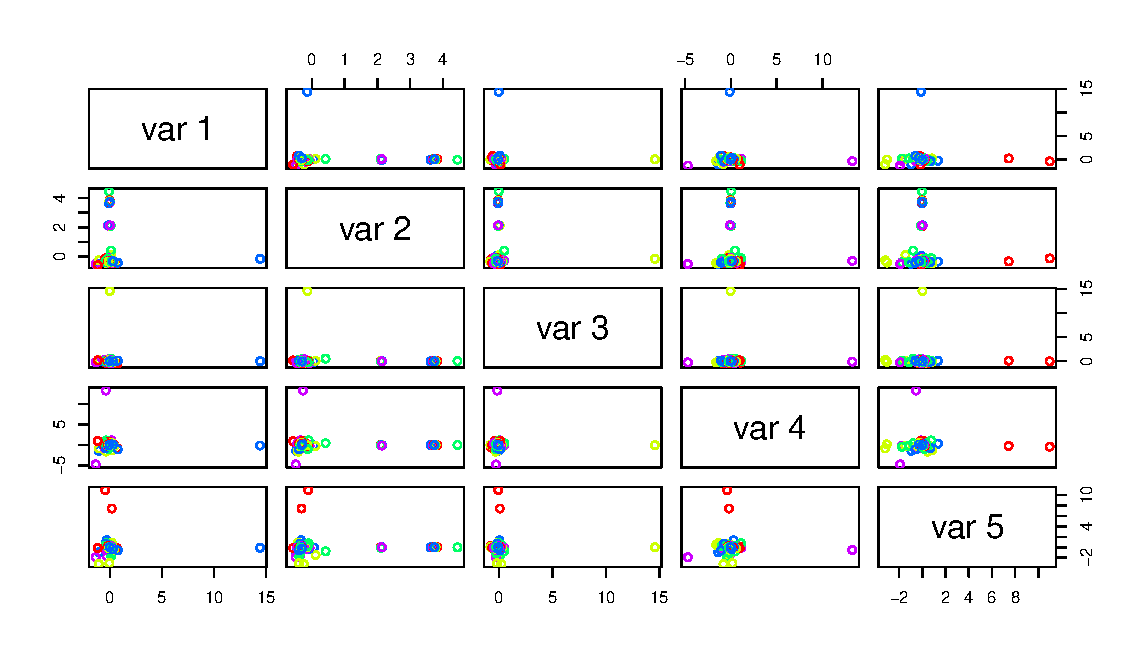
\includegraphics[width=15cm]{images/ICA/[5]/[5] 5 x 5 plot.pdf}  
    \caption{Biplots of 5 components}
    \label{fig:[5]5x5biplots]} 
\end{figure}

It is unclear to tell which component best separates the data on its own, or in other words is closest to a uniform shape, just by observing the biplots. In order to determine which component best separates the data, we can compute the difference of the 219 elements of each component to a uniform vector of same maximum and minimum value and number of points.

For each i-th component, which can be accessed as \emph{S}[,i], we calculate the sum of the absolute value of the difference between each element from a uniform matrix and the closest element from the i-th component. 

By using a \emph{for}() loop with variable \emph{j} from 1 to 219, we calculate the element of i-th component which is the closest to the j-th index element of the uniform vector. Then we calculate the absolute value of the difference of the two values. Throughout the iteration, we increment these 219 values into object \emph{uniVal}. Thus, we have the total sum of the difference \emph{uniVal} for each i-th component.

The component with the lowest \emph{uniVal} value would be the one that is the closest to a uniform distribution. Using this algorithm on data \emph{ica5}, we get a result that component 2 has the lowest \emph{uniVal} value. We can plot a representation of component 2 to observe and visually confirm the spread and variance. The following figure is a biplot with x and y axis both being component 2, \emph{S}[,2].
\begin{figure}[H]
    \centering
    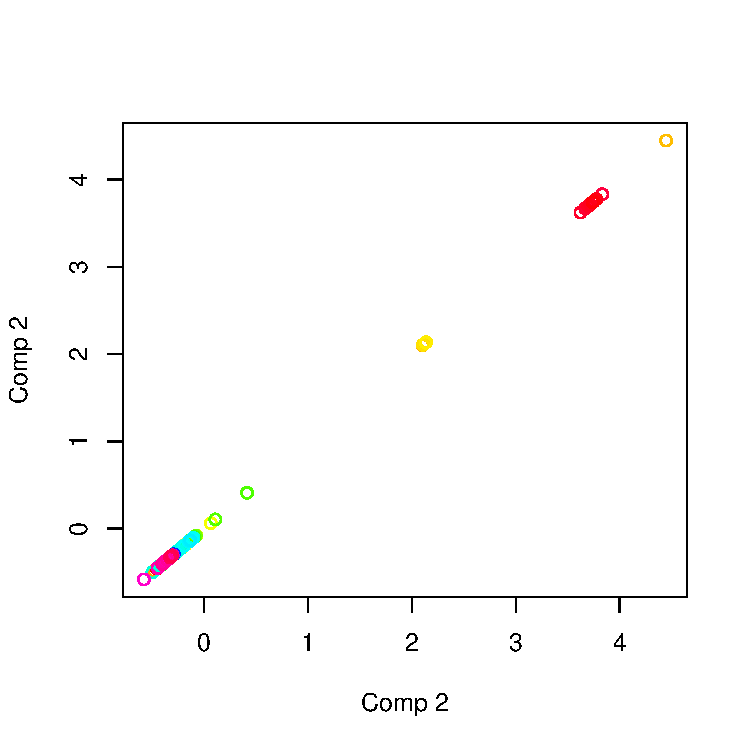
\includegraphics[width=9cm]{images/ICA/[5]/comp 2.pdf}  
    \caption{Biplot of component 2}
    \label{fig:[5]comp2} 
\end{figure}

Now we can increase the value of \emph{n.comp} and observe the difference in the result. We execute \emph{fastICA} with \emph{n.comp} set as 10 and save the computed result in object \emph{ica10}. Using the same algorithm to calculate which component best separates the data on its own, we get a result that component 19 has the lowest \emph{uniVal} value. The following figure is a biplot with x and y axis both being component 19, \emph{S}[,19].
\begin{figure}[H]
    \centering
    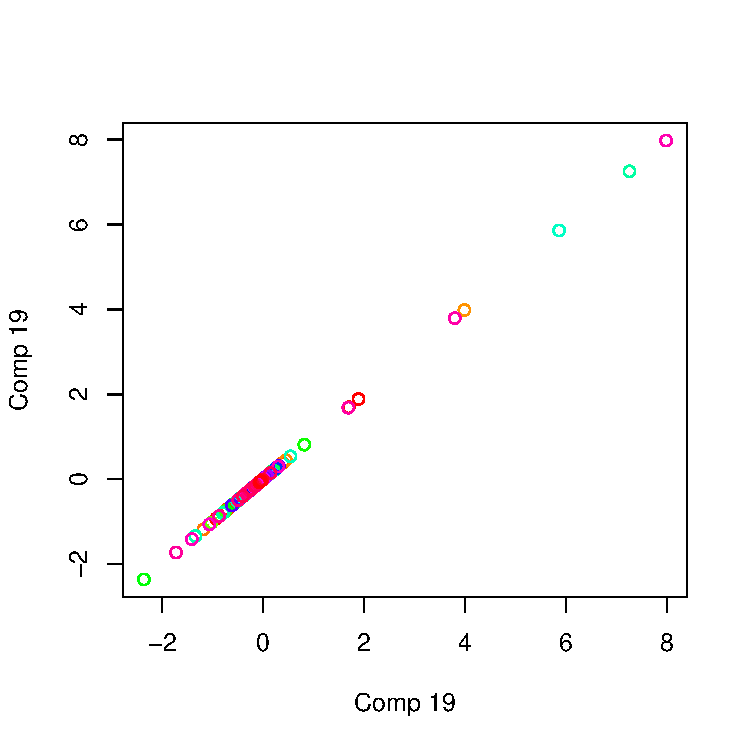
\includegraphics[width=9cm]{images/ICA/[10]/comp 19.pdf}  
    \caption{Biplot of component 19}
    \label{fig:[10]comp19} 
\end{figure}
We can notice from the figure that the plot of component 19 from \emph{ica10} is more evenly distributed and has a shape closer to a uniform vector, compared to the plot of component 2 from \emph{ica5}. From this result we can assume that increasing the value of \emph{n.comp} leads to increased number of components being produced, thus may lead to finding a better representation of component that best separates the data on its own. We would carry on with further exectuion of \emph{fastICA} with increased value of \emph{n.comp} in order to verify this assumption.

Again, we execute \emph{fastICA} with increased value of \emph{n.comp}, set to 20, and save the computed result in object \emph{ica20}. Using the same algorithm to calculate which component best separates the data on its own, we get a result that component 7 has the lowest \emph{uniVal} value. The following figure is a biplot with x and y axis both being component 7, \emph{S}[,7].
\begin{figure}[H]
    \centering
    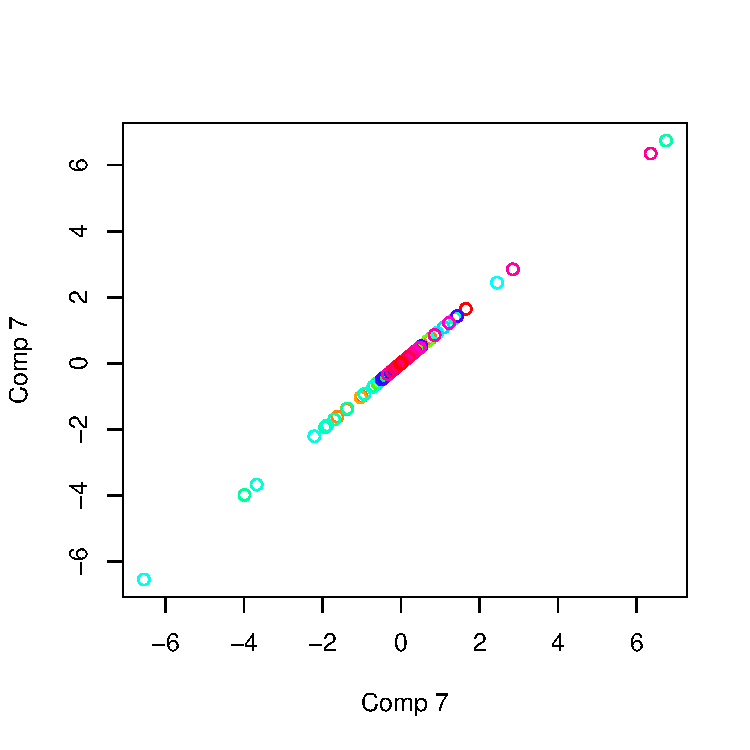
\includegraphics[width=9cm]{images/ICA/[20]/comp 7.pdf}  
    \caption{Biplot of component 7}
    \label{fig:[20]comp7} 
\end{figure}

Again, we execute \emph{fastICA} with increased value of \emph{n.comp}, set to 40, and save the computed result in object \emph{ica40}. Using the same algorithm to calculate which component best separates the data on its own, we get a result that component 13 has the lowest \emph{uniVal} value. The following figure is a biplot with x and y axis both being component 13, \emph{S}[,13].
\begin{figure}[H]
    \centering
    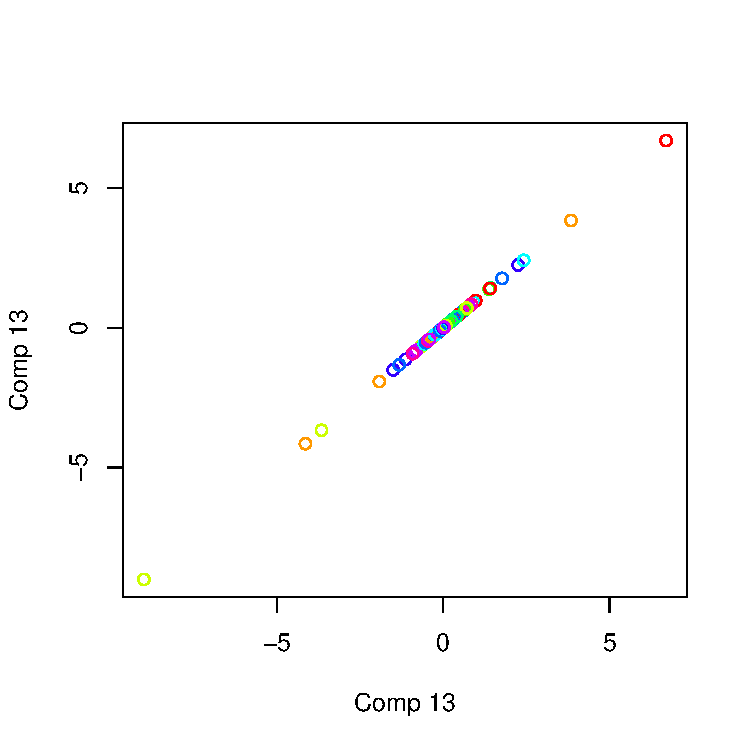
\includegraphics[width=9cm]{images/ICA/[40]/comp 13.pdf}  
    \caption{Biplot of component 13}
    \label{fig:[40]comp13} 
\end{figure}

We execute our last process of \emph{fastICA} with increased value of \emph{n.comp}, set to 80, and save the computed result in object \emph{ica80}. Using the same algorithm to calculate which component best separates the data on its own, we get a result that component 50 has the lowest \emph{uniVal} value. The following figure is a biplot with x and y axis both being component 50, \emph{S}[,50].
\begin{figure}[H]
    \centering
    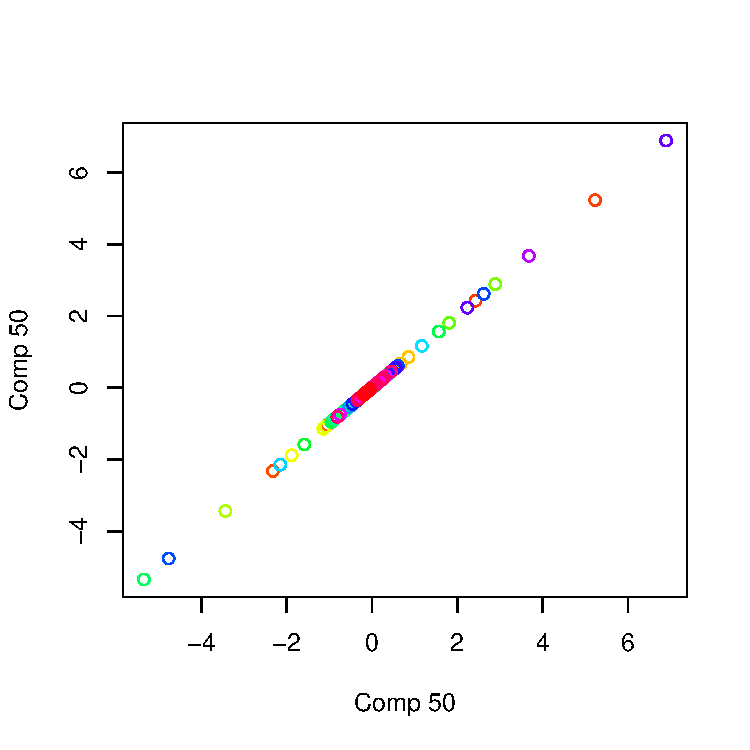
\includegraphics[width=9cm]{images/ICA/[80]/comp 50.pdf}  
    \caption{Biplot of component 50}
    \label{fig:[80]comp50} 
\end{figure}

By comparing the five biplots of the best separating components from each processed data \emph{ica5, ica10, ica20, ica40, ica80}, we can observe that throughout each iteration, as the value set for \emph{n.comp} increases, the plot forms closer to a uniform vector.

In conclusion we have applied the \emph{fastICA} algorithm on interpolated 219 acoustic signal data with five different values selected for the number of components. We have made an assumption that as the number of components calculated increases, the more likely we could find a component that well-separates the data on its own. Throughout the 5 calculations, from 5 components to 80 components, we have visually observed through the biplots of the components that our assumption holds valid.

Application of \emph{fastICA} on spectrum dataframe could not have been performed due to the exhausting time complexity of the data. This aspect also shows the inefficiency of ICA algorithms, when it is used with the goal to reduce the dimension of acoustic signal data with large number of sampling points (in other words variables), rather than to separate independent sources from a mixed signal. 
\newpage
\section{Summary}


Throughout this dissertation we have introduced the fundamentals of dimensional reduction and demonstrated practical application via R language on acoustic signals.

We have thoroughly introduced two major dimensional reduction techniques: principal component analysis (PCA) and independent component analysis (ICA). We have narrated the general characteristics, mathematical definitions, and applicational process of both techniques with real-life examples and precise logical reasoning.

We have introduced and shown several pre-processing of data, such as interpolation, centering, whitening, etc... , by actual demonstration on 219 acoustic signals of Romance languages via R language. We have also narrated and demonstrated the transformation of the processed data into spectrum and have produced visual representation as spectrograms.

Lastly, we have successfully implemented the PCA and ICA techniques on the processed data and deliberately analyzed the results with various visual representations. 

We have applied the PCA method on interpolated data, spectrum data, and on data sorted by different types of languages. We have carefully executed each process with deliberate coding and have successfully narrated the numeric results of each progress.

We have applied the ICA method on interpolated data on various input conditions, and have well-plotted the visual representations of the results. We have affirmed our initial assumption on the effectiveness of components throughout the five computation process.

By analyzing the numeric and visual results from both methods, we can conclude that the PCA method is more suitable and efficient when performing dimensional reduction on acoustic signal data, which has a substantially high volume of variables (or in other words dimensions). We approached a result of 84 percent reduction in dimension with 80 percent of total variance for spectrum dataframe, and 64 percent reduction in dimension with 90 percent of total variance for interpolated dataframe.

In conclusion, the following dissertation well-explained the fundamentals of dimensional reduction and thoroughly demonstrated the application of the dimensional techniques on acoustic signals via R language.




\newpage
\section*{Appendix}


In this section we will show the actual code lines used for this dissertation

This is the code used for interpolating the original Romance Digit data file into a dataframe and plotting relevant figures.
\begin{verbatim}
########## Interpolation ############


itpData <- matrix(0, ncol = 5000, nrow = 1)

for (i in 1:length(Data)){
  ytemp <- data.frame(Data[i])
  y <- c()
  
  for (j in 1:nrow(ytemp)){
    y <- append(y, ytemp[j,])
  }
  
  x <- c(1:nrow(ytemp))
  
  ##plot(x, y)
  
  xoutval = seq(1,nrow(ytemp),len=5000)
  templist <- approx(x, y, xout=xoutval, method='linear')
  
  ##plot(templist)
  
  tempylist <- unlist(templist[2])
  itpData <- rbind(itpData, tempylist)
}

finalDF <- data.frame(itpData)
finalDF <- finalDF[-1, ]

for (i in 1:nrow(finalDF)){
  rownames(finalDF)[i] <- names(Data)[i]
}

saveDF <- finalDF

rm(itpData)
rm(my_pca)
rm(templist)
rm(ytemp)
\end{verbatim}

This is the code used for transforming the interpolated dataframe into a spectrum and plotting relevant figures such as spectrograms
\begin{verbatim}
################## Spectrogram ################


library(signal, warn.conflicts = F, quietly = T) # signal processing functions
library(oce, warn.conflicts = F, quietly = T) # image plotting functions and nice color maps
library(tuneR, warn.conflicts = F, quietly = T) 

specData <- matrix(0, ncol = 19456, nrow = 1)

nfft=1024
window=256
overlap=128
dur=5
fs=1000

for (i in 1:length(Data)){
  snd = unlist(finalDF[i,])
  mean(snd)
  snd = snd - mean(snd)
  
  setwd("C:/Users/csia7/Desktop/OneDrive/OneDrive_2022-11-08/6CCM345A Third Year Project/R/R images/Spectrum(new)/Romance/Wave")
  pdf(paste(gsub("c", "", rownames(finalDF)[i]), "pdf", sep=""), width = 15, height = 8) 
  plot(snd, type = 'l', xlab = 'Samples', ylab = 'Amplitude')
  dev.off() 
  
  spec = specgram(x = snd, n = nfft, Fs = fs, window = window, overlap = overlap)
  
  P = abs(spec$S)
  P = P/max(P)
  P = 10*log10(P)
  t = spec$t
  
  setwd("C:/Users/csia7/Desktop/OneDrive/OneDrive_2022-11-08/6CCM345A Third Year Project/R/R images/Spectrum(new)/Romance/Spectrogram (raw)")
  pdf(paste(gsub("c", "", rownames(finalDF)[i]), "pdf", sep=""), width = 15, height = 8) 
  image(P)
  dev.off() 
  
  setwd("C:/Users/csia7/Desktop/OneDrive/OneDrive_2022-11-08/6CCM345A Third Year Project/R/R images/Spectrum(new)/Romance/Spectrogram (processed)")
  pdf(paste(gsub("c", "", rownames(finalDF)[i]), "pdf", sep=""), width = 15, height = 8) 
  imagep(x = t, y = spec$f, z = t(P), col = oce.colorsViridis, ylab = 'Frequency [Hz]', xlab = 'Time [s]', drawPalette = T, decimate = F
  )
  dev.off()
  
  P <- c(t(P))
  specData <- rbind(specData, P)
}

finalSpec <- data.frame(specData)
finalSpec <- finalSpec[-1, ]

for (i in 1:nrow(finalSpec)){
  rownames(finalSpec)[i] <- names(Data)[i]
}

saveSpec <- finalSpec

rm(spec)
rm(specData)
\end{verbatim}

This is the code used for applying the PCA technique on interpolated dataframe and plotting relevant figures.
\begin{verbatim}
###################### PCA #####################


help(prcomp)
library(factoextra)

my_pca <- prcomp(finalDF, scale = TRUE, center = TRUE, retx = T)

names(my_pca);
summary(my_pca);

my_pca$sdev
my_pca$rotation
my_pca$center
my_pca$scale
my_pca$x
dim(my_pca$x);

setwd("C:/Users/csia7/Desktop/OneDrive/OneDrive_2022-11-08/6CCM345A Third Year Project/R/R images/PCA/rotations")
pdf("PC1 rotation.pdf", width = 15, height = 8) 
plot(my_pca$rotation[,1], type = "l", xlab = "PC1", ylab = "rotation")
dev.off()

pdf("PC2 rotation.pdf", width = 15, height = 8) 
plot(my_pca$rotation[,2], type = "l", xlab = "PC2", ylab = "rotation")
dev.off()

pdf("PC3 rotation.pdf", width = 15, height = 8) 
plot(my_pca$rotation[,3], type = "l", xlab = "PC3", ylab = "rotation")
dev.off()

setwd("C:/Users/csia7/Desktop/OneDrive/OneDrive_2022-11-08/6CCM345A Third Year Project/R/R images/PCA/PC biplots")
pdf("PC1 and PC2.pdf", width = 15, height = 8) 
plot(my_pca$x[,1], my_pca$x[,2], cex = 1, xlab = "PC1", ylab = "PC2", main = "PC1 and PC2")
dev.off()

pdf("PC1 and PC3.pdf", width = 15, height = 8) 
plot(my_pca$x[,1], my_pca$x[,3], cex = 1, xlab = "PC1", ylab = "PC3", main = "PC1 and PC3")
dev.off()

pdf("PC2 and PC3.pdf", width = 15, height = 8) 
plot(my_pca$x[,2], my_pca$x[,3], cex = 1, xlab = "PC2", ylab = "PC3", main = "PC2 and PC3")
dev.off()

# Compute variance

my_pca.var <- my_pca$sdev ^ 2;
my_pca.var;

# Proportion of variance for a scree plot #

propve <- my_pca.var / sum(my_pca.var);
propve;

setwd("C:/Users/csia7/Desktop/OneDrive/OneDrive_2022-11-08/6CCM345A Third Year Project/R/R images/PCA/Scree Plot")
pdf("Scree Plot.pdf", width = 15, height = 8) 
plot(propve, xlab = "Principal Component",
     ylab = "Proportion of Variance",
     ylim = c(0, 1), type = "b",
     main = "Scree Plot");
dev.off()

# Plot the cumulative proportion of variance explained

pdf("Cumulative Scree Plot.pdf", width = 15, height = 8) 
plot(cumsum(propve),
     xlab = "Principal Component",
     ylab = "Cumulative Proportion of Variance",
     ylim = c(0, 1), 
     type = "b",
     main = "Cumulative Scree Plot");
dev.off()

#Find Top n principal component
# which will at least cover 90 % variance of dimension

dim(my_pca$x) # 219
ncovdata <- which(cumsum(propve) >= 0.8)[1] 
ncovdata # 56/219
ncovdata <- which(cumsum(propve) >= 0.9)[1] 
ncovdata # 85/219
ncovdata <- which(cumsum(propve) >= 0.95)[1] 
ncovdata # 112/219

rm(my_pca)
\end{verbatim}

This is the code used for applying the PCA technique on spectrum dataframe and plotting relevant figures.
\begin{verbatim}
################### PCA on Spectrum ################


my_pca <- prcomp(finalSpec, scale = TRUE, center = TRUE, retx = T)

names(my_pca);
summary(my_pca);

my_pca$sdev
my_pca$rotation
my_pca$center
my_pca$scale
my_pca$x
dim(my_pca$x);

setwd("C:/Users/csia7/Desktop/OneDrive/OneDrive_2022-11-08/6CCM345A Third Year Project/R/R images/PCA Spectrum/rotations")
pdf("PC1 rotation.pdf", width = 15, height = 8) 
plot(my_pca$rotation[,1], type = "l", xlab = "PC1", ylab = "rotation")
dev.off()

pdf("PC2 rotation.pdf", width = 15, height = 8) 
plot(my_pca$rotation[,2], type = "l", xlab = "PC2", ylab = "rotation")
dev.off()

pdf("PC3 rotation.pdf", width = 15, height = 8) 
plot(my_pca$rotation[,3], type = "l", xlab = "PC3", ylab = "rotation")
dev.off()

setwd("C:/Users/csia7/Desktop/OneDrive/OneDrive_2022-11-08/6CCM345A Third Year Project/R/R images/PCA Spectrum/PC biplots")
pdf("PC1 and PC2.pdf", width = 15, height = 8) 
plot(my_pca$x[,1], my_pca$x[,2], cex = 1, xlab = "PC1", ylab = "PC2", main = "PC1 and PC2")
dev.off()

pdf("PC1 and PC3.pdf", width = 15, height = 8) 
plot(my_pca$x[,1], my_pca$x[,3], cex = 1, xlab = "PC1", ylab = "PC3", main = "PC1 and PC3")
dev.off()

pdf("PC2 and PC3.pdf", width = 15, height = 8) 
plot(my_pca$x[,2], my_pca$x[,3], cex = 1, xlab = "PC2", ylab = "PC3", main = "PC2 and PC3")
dev.off()

# Compute variance

my_pca.var <- my_pca$sdev ^ 2;
my_pca.var;

# Proportion of variance for a scree plot

propve <- my_pca.var / sum(my_pca.var);
propve;

setwd("C:/Users/csia7/Desktop/OneDrive/OneDrive_2022-11-08/6CCM345A Third Year Project/R/R images/PCA Spectrum/Scree Plot")
pdf("Scree Plot.pdf", width = 15, height = 8) 
plot(propve, xlab = "Principal Component",
     ylab = "Proportion of Variance",
     ylim = c(0, 1), type = "b",
     main = "Scree Plot");
dev.off()

# Plot the cumulative proportion of variance explained

pdf("Cumulative Scree Plot.pdf", width = 15, height = 8) 
plot(cumsum(propve),
     xlab = "Principal Component",
     ylab = "Cumulative Proportion of Variance",
     ylim = c(0, 1), 
     type = "b",
     main = "Cumulative Scree Plot");
dev.off()

# Find Top n principal component
# which will atleast cover 90 % variance of dimension

ncovdata <- which(cumsum(propve) >= 0.8)[1] 
ncovdata # 35
ncovdata <- which(cumsum(propve) >= 0.9)[1] 
ncovdata # 92
ncovdata <- which(cumsum(propve) >= 0.95)[1] 
ncovdata # 142
\end{verbatim}

This is the code used for applying the PCA technique on Portuguese section of the interpolated dataframe and plotting relevant figures.
\begin{verbatim}
######################## PCA (Portuguese) ########################


library(dplyr)

finalDFPO <- finalDF[1:25, ]
finalDFPOM <- finalDF[1:9, ]
finalDFPOF <- finalDF[10:25, ]

my_pca <- prcomp(finalDFPO, scale = TRUE, center = TRUE, retx = T)

names(my_pca);
summary(my_pca);

my_pca$sdev
my_pca$rotation
my_pca$center
my_pca$scale
my_pca$x
dim(my_pca$x);

setwd("C:/Users/csia7/Desktop/OneDrive/OneDrive_2022-11-08/6CCM345A Third Year Project/R/R images/PCA (Portuguese)/rotations")
pdf("PC1 rotation.pdf", width = 15, height = 8) 
plot(my_pca$rotation[,1], type = "l", xlab = "PC1", ylab = "rotation")
dev.off()

pdf("PC2 rotation.pdf", width = 15, height = 8) 
plot(my_pca$rotation[,2], type = "l", xlab = "PC2", ylab = "rotation")
dev.off()

pdf("PC3 rotation.pdf", width = 15, height = 8) 
plot(my_pca$rotation[,3], type = "l", xlab = "PC3", ylab = "rotation")
dev.off()

setwd("C:/Users/csia7/Desktop/OneDrive/OneDrive_2022-11-08/6CCM345A Third Year Project/R/R images/PCA (Portuguese)/PC biplots")
pdf("PC1 and PC2.pdf", width = 15, height = 8) 
plot(my_pca$x[,1], my_pca$x[,2], cex = 1, xlab = "PC1", ylab = "PC2", main = "PC1 and PC2")
dev.off()

pdf("PC1 and PC3.pdf", width = 15, height = 8) 
plot(my_pca$x[,1], my_pca$x[,3], cex = 1, xlab = "PC1", ylab = "PC3", main = "PC1 and PC3")
dev.off()

pdf("PC2 and PC3.pdf", width = 15, height = 8) 
plot(my_pca$x[,2], my_pca$x[,3], cex = 1, xlab = "PC2", ylab = "PC3", main = "PC2 and PC3")
dev.off()

# Compute variance

my_pca.var <- my_pca$sdev ^ 2;
my_pca.var;

# Proportion of variance for a scree plot

propve <- my_pca.var / sum(my_pca.var);
propve;

setwd("C:/Users/csia7/Desktop/OneDrive/OneDrive_2022-11-08/6CCM345A Third Year Project/R/R images/PCA (Portuguese)/Scree Plot")
pdf("Scree Plot.pdf", width = 15, height = 8) 
plot(propve, xlab = "Principal Component",
     ylab = "Proportion of Variance",
     ylim = c(0, 1), type = "b",
     main = "Scree Plot");
dev.off()

# Plot the cumulative proportion of variance explained

pdf("Cumulative Scree Plot.pdf", width = 15, height = 8) 
plot(cumsum(propve),
     xlab = "Principal Component",
     ylab = "Cumulative Proportion of Variance",
     ylim = c(0, 1), 
     type = "b",
     main = "Cumulative Scree Plot");
dev.off()

# Find Top n principal component
# which will at least cover 90 % variance of dimension

dim(my_pca$x) # 25
ncovdata <- which(cumsum(propve) >= 0.8)[1] 
ncovdata # 14/25
ncovdata <- which(cumsum(propve) >= 0.9)[1] 
ncovdata # 17/25
ncovdata <- which(cumsum(propve) >= 0.95)[1] 
ncovdata # 20/25
\end{verbatim}

This is the code used for applying the PCA technique on Italian section of the interpolated dataframe and plotting relevant figures.
\begin{verbatim}
######################## PCA (Italian) ########################

library(dplyr)

finalDFIT <- finalDF[26:75, ]

my_pca <- prcomp(finalDFIT, scale = TRUE, center = TRUE, retx = T)

names(my_pca);
summary(my_pca);

my_pca$sdev
my_pca$rotation
my_pca$center
my_pca$scale
my_pca$x
dim(my_pca$x);

setwd("C:/Users/csia7/Desktop/OneDrive/OneDrive_2022-11-08/6CCM345A Third Year Project/R/R images/PCA (Italian)/rotations")
pdf("PC1 rotation.pdf", width = 15, height = 8) 
plot(my_pca$rotation[,1], type = "l", xlab = "PC1", ylab = "rotation")
dev.off()

pdf("PC2 rotation.pdf", width = 15, height = 8) 
plot(my_pca$rotation[,2], type = "l", xlab = "PC2", ylab = "rotation")
dev.off()

pdf("PC3 rotation.pdf", width = 15, height = 8) 
plot(my_pca$rotation[,3], type = "l", xlab = "PC3", ylab = "rotation")
dev.off()

setwd("C:/Users/csia7/Desktop/OneDrive/OneDrive_2022-11-08/6CCM345A Third Year Project/R/R images/PCA (Italian)/PC biplots")
pdf("PC1 and PC2.pdf", width = 15, height = 8) 
plot(my_pca$x[,1], my_pca$x[,2], cex = 1, xlab = "PC1", ylab = "PC2", main = "PC1 and PC2")
dev.off()

pdf("PC1 and PC3.pdf", width = 15, height = 8) 
plot(my_pca$x[,1], my_pca$x[,3], cex = 1, xlab = "PC1", ylab = "PC3", main = "PC1 and PC3")
dev.off()

pdf("PC2 and PC3.pdf", width = 15, height = 8) 
plot(my_pca$x[,2], my_pca$x[,3], cex = 1, xlab = "PC2", ylab = "PC3", main = "PC2 and PC3")
dev.off()

# Compute variance

my_pca.var <- my_pca$sdev ^ 2;
my_pca.var;

# Proportion of variance for a scree plot

propve <- my_pca.var / sum(my_pca.var);
propve;

setwd("C:/Users/csia7/Desktop/OneDrive/OneDrive_2022-11-08/6CCM345A Third Year Project/R/R images/PCA (Italian)/Scree Plot")
pdf("Scree Plot.pdf", width = 15, height = 8) 
plot(propve, xlab = "Principal Component",
     ylab = "Proportion of Variance",
     ylim = c(0, 1), type = "b",
     main = "Scree Plot");
dev.off()

# Plot the cumulative proportion of variance explained

pdf("Cumulative Scree Plot.pdf", width = 15, height = 8) 
plot(cumsum(propve),
     xlab = "Principal Component",
     ylab = "Cumulative Proportion of Variance",
     ylim = c(0, 1), 
     type = "b",
     main = "Cumulative Scree Plot");
dev.off()

# Find Top n principal component
# which will at least cover 90 % variance of dimension

dim(my_pca$x) # 50
ncovdata <- which(cumsum(propve) >= 0.8)[1] 
ncovdata # 20/50
ncovdata <- which(cumsum(propve) >= 0.9)[1] 
ncovdata # 29/50
ncovdata <- which(cumsum(propve) >= 0.95)[1] 
ncovdata # 35/50
\end{verbatim}

This is the code used for applying the PCA technique on Spanish Italian section of the interpolated dataframe and plotting relevant figures.
\begin{verbatim}
##################### PCA (Spanish Italian) #####################


library(dplyr)

finalDFSI <- finalDF[76:113, ]
finalDFSIM <- finalDF[85:94, ]
finalDFSIM <- bind_rows(finalDFSIM, finalDF[104:113, ])
finalDFSIF <- finalDF[76:84, ]
finalDFSIF <- bind_rows(finalDFSIF, finalDF[95:103, ])

dim(finalDFSI)
dim(finalDFSIM)
dim(finalDFSIF)

my_pca <- prcomp(finalDFSI, scale = TRUE, center = TRUE, retx = T)

names(my_pca);
summary(my_pca);

my_pca$sdev
my_pca$rotation
my_pca$center
my_pca$scale
my_pca$x
dim(my_pca$x);

setwd("C:/Users/csia7/Desktop/OneDrive/OneDrive_2022-11-08/6CCM345A Third Year Project/R/R images/PCA (Iberian Spanish)/rotations")
pdf("PC1 rotation.pdf", width = 15, height = 8) 
plot(my_pca$rotation[,1], type = "l", xlab = "PC1", ylab = "rotation")
dev.off()

pdf("PC2 rotation.pdf", width = 15, height = 8) 
plot(my_pca$rotation[,2], type = "l", xlab = "PC2", ylab = "rotation")
dev.off()

pdf("PC3 rotation.pdf", width = 15, height = 8) 
plot(my_pca$rotation[,3], type = "l", xlab = "PC3", ylab = "rotation")
dev.off()

setwd("C:/Users/csia7/Desktop/OneDrive/OneDrive_2022-11-08/6CCM345A Third Year Project/R/R images/PCA (Iberian Spanish)/PC biplots")
pdf("PC1 and PC2.pdf", width = 15, height = 8) 
plot(my_pca$x[,1], my_pca$x[,2], cex = 1, xlab = "PC1", ylab = "PC2", main = "PC1 and PC2")
dev.off()

pdf("PC1 and PC3.pdf", width = 15, height = 8) 
plot(my_pca$x[,1], my_pca$x[,3], cex = 1, xlab = "PC1", ylab = "PC3", main = "PC1 and PC3")
dev.off()

pdf("PC2 and PC3.pdf", width = 15, height = 8) 
plot(my_pca$x[,2], my_pca$x[,3], cex = 1, xlab = "PC2", ylab = "PC3", main = "PC2 and PC3")
dev.off()

# Compute variance

my_pca.var <- my_pca$sdev ^ 2;
my_pca.var;

# Proportion of variance for a scree plot

propve <- my_pca.var / sum(my_pca.var);
propve;

setwd("C:/Users/csia7/Desktop/OneDrive/OneDrive_2022-11-08/6CCM345A Third Year Project/R/R images/PCA (Iberian Spanish)/Scree Plot")
pdf("Scree Plot.pdf", width = 15, height = 8) 
plot(propve, xlab = "Principal Component",
     ylab = "Proportion of Variance",
     ylim = c(0, 1), type = "b",
     main = "Scree Plot");
dev.off()

# Plot the cumulative proportion of variance explained

pdf("Cumulative Scree Plot.pdf", width = 15, height = 8) 
plot(cumsum(propve),
     xlab = "Principal Component",
     ylab = "Cumulative Proportion of Variance",
     ylim = c(0, 1), 
     type = "b",
     main = "Cumulative Scree Plot");
dev.off()

# Find Top n principal component
# which will at least cover 90 % variance of dimension

dim(my_pca$x) # 38
ncovdata <- which(cumsum(propve) >= 0.8)[1] 
ncovdata # 15/38
ncovdata <- which(cumsum(propve) >= 0.9)[1] 
ncovdata # 21/38
ncovdata <- which(cumsum(propve) >= 0.95)[1] 
ncovdata # 26/38
\end{verbatim}

This is the code used for applying the PCA technique on French section of the interpolated dataframe and plotting relevant figures.
\begin{verbatim}
######################## PCA (French) ########################


library(dplyr)

finalDFFR <- finalDF[114:173, ]
finalDFFRM <- finalDF[134:143, ]
finalDFFRM <- bind_rows(finalDFFRM, finalDF[160:163, ])
finalDFFRF <- finalDF[114:133, ]
finalDFFRF <- bind_rows(finalDFFRF, finalDF[144:159, ])
finalDFFRF <- bind_rows(finalDFFRF, finalDF[164:173, ])

dim(finalDFFR)
dim(finalDFFRM)
dim(finalDFFRF)

my_pca <- prcomp(finalDFFR, scale = TRUE, center = TRUE, retx = T)

names(my_pca);
summary(my_pca);

my_pca$sdev
my_pca$rotation
my_pca$center
my_pca$scale
my_pca$x
dim(my_pca$x);

setwd("C:/Users/csia7/Desktop/OneDrive/OneDrive_2022-11-08/6CCM345A Third Year Project/R/R images/PCA (French)/rotations")
pdf("PC1 rotation.pdf", width = 15, height = 8) 
plot(my_pca$rotation[,1], type = "l", xlab = "PC1", ylab = "rotation")
dev.off()

pdf("PC2 rotation.pdf", width = 15, height = 8) 
plot(my_pca$rotation[,2], type = "l", xlab = "PC2", ylab = "rotation")
dev.off()

pdf("PC3 rotation.pdf", width = 15, height = 8) 
plot(my_pca$rotation[,3], type = "l", xlab = "PC3", ylab = "rotation")
dev.off()

setwd("C:/Users/csia7/Desktop/OneDrive/OneDrive_2022-11-08/6CCM345A Third Year Project/R/R images/PCA (French)/PC biplots")
pdf("PC1 and PC2.pdf", width = 15, height = 8) 
plot(my_pca$x[,1], my_pca$x[,2], cex = 1, xlab = "PC1", ylab = "PC2", main = "PC1 and PC2")
dev.off()

pdf("PC1 and PC3.pdf", width = 15, height = 8) 
plot(my_pca$x[,1], my_pca$x[,3], cex = 1, xlab = "PC1", ylab = "PC3", main = "PC1 and PC3")
dev.off()

pdf("PC2 and PC3.pdf", width = 15, height = 8) 
plot(my_pca$x[,2], my_pca$x[,3], cex = 1, xlab = "PC2", ylab = "PC3", main = "PC2 and PC3")
dev.off()

# Compute variance

my_pca.var <- my_pca$sdev ^ 2;
my_pca.var;

# Proportion of variance for a scree plot

propve <- my_pca.var / sum(my_pca.var);
propve;

setwd("C:/Users/csia7/Desktop/OneDrive/OneDrive_2022-11-08/6CCM345A Third Year Project/R/R images/PCA (French)/Scree Plot")
pdf("Scree Plot.pdf", width = 15, height = 8) 
plot(propve, xlab = "Principal Component",
     ylab = "Proportion of Variance",
     ylim = c(0, 1), type = "b",
     main = "Scree Plot");
dev.off()

# Plot the cumulative proportion of variance explained

pdf("Cumulative Scree Plot.pdf", width = 15, height = 8) 
plot(cumsum(propve),
     xlab = "Principal Component",
     ylab = "Cumulative Proportion of Variance",
     ylim = c(0, 1), 
     type = "b",
     main = "Cumulative Scree Plot");
dev.off()

# Find Top n principal component
# which will at least cover 90 % variance of dimension

dim(my_pca$x) # 60
ncovdata <- which(cumsum(propve) >= 0.8)[1] 
ncovdata # 22/60
ncovdata <- which(cumsum(propve) >= 0.9)[1] 
ncovdata # 31/60
ncovdata <- which(cumsum(propve) >= 0.95)[1] 
ncovdata # 39/60
\end{verbatim}

This is the code used for applying the PCA technique on American Spanish section of the interpolated dataframe and plotting relevant figures.
\begin{verbatim}
##################### PCA (American Spanish) #####################

library(dplyr)

finalDFSA <- finalDF[174:219, ]
finalDFSAM <- finalDF[180:189, ]
finalDFSAF <- finalDF[174:179, ]
finalDFSAF <- bind_rows(finalDFSAF, finalDF[190:219, ])

dim(finalDFSA)
dim(finalDFSAM)
dim(finalDFSAF)

my_pca <- prcomp(finalDFSA, scale = TRUE, center = TRUE, retx = T)

names(my_pca);
summary(my_pca);

my_pca$sdev
my_pca$rotation
my_pca$center
my_pca$scale
my_pca$x
dim(my_pca$x);

setwd("C:/Users/csia7/Desktop/OneDrive/OneDrive_2022-11-08/6CCM345A Third Year Project/R/R images/PCA (American Spanish)/rotations")
pdf("PC1 rotation.pdf", width = 15, height = 8) 
plot(my_pca$rotation[,1], type = "l", xlab = "PC1", ylab = "rotation")
dev.off()

pdf("PC2 rotation.pdf", width = 15, height = 8) 
plot(my_pca$rotation[,2], type = "l", xlab = "PC2", ylab = "rotation")
dev.off()

pdf("PC3 rotation.pdf", width = 15, height = 8) 
plot(my_pca$rotation[,3], type = "l", xlab = "PC3", ylab = "rotation")
dev.off()

setwd("C:/Users/csia7/Desktop/OneDrive/OneDrive_2022-11-08/6CCM345A Third Year Project/R/R images/PCA (American Spanish)/PC biplots")
pdf("PC1 and PC2.pdf", width = 15, height = 8) 
plot(my_pca$x[,1], my_pca$x[,2], cex = 1, xlab = "PC1", ylab = "PC2", main = "PC1 and PC2")
dev.off()

pdf("PC1 and PC3.pdf", width = 15, height = 8) 
plot(my_pca$x[,1], my_pca$x[,3], cex = 1, xlab = "PC1", ylab = "PC3", main = "PC1 and PC3")
dev.off()

pdf("PC2 and PC3.pdf", width = 15, height = 8) 
plot(my_pca$x[,2], my_pca$x[,3], cex = 1, xlab = "PC2", ylab = "PC3", main = "PC2 and PC3")
dev.off()

# Compute variance

my_pca.var <- my_pca$sdev ^ 2;
my_pca.var;

# Proportion of variance for a scree plot

propve <- my_pca.var / sum(my_pca.var);
propve;

setwd("C:/Users/csia7/Desktop/OneDrive/OneDrive_2022-11-08/6CCM345A Third Year Project/R/R images/PCA (American Spanish)/Scree Plot")
pdf("Scree Plot.pdf", width = 15, height = 8) 
plot(propve, xlab = "Principal Component",
     ylab = "Proportion of Variance",
     ylim = c(0, 1), type = "b",
     main = "Scree Plot");
dev.off()

# Plot the cumulative proportion of variance explained

pdf("Cumulative Scree Plot.pdf", width = 15, height = 8) 
plot(cumsum(propve),
     xlab = "Principal Component",
     ylab = "Cumulative Proportion of Variance",
     ylim = c(0, 1), 
     type = "b",
     main = "Cumulative Scree Plot");
dev.off()

# Find Top n principal component
# which will at least cover 90 % variance of dimension

dim(my_pca$x) # 46
ncovdata <- which(cumsum(propve) >= 0.8)[1] 
ncovdata # 7/46
ncovdata <- which(cumsum(propve) >= 0.9)[1] 
ncovdata # 11/46
ncovdata <- which(cumsum(propve) >= 0.95)[1] 
ncovdata # 18/46
\end{verbatim}

This is the code used for applying the ICA technique on the interpolated dataframe and plotting relevant figures.
\begin{verbatim}
###################### ICA ####################


install.packages("fastICA")
install.packages("scatterplot3d")
library(fastICA)
library(scatterplot3d)

# ICA with n.comp=5 

ica5 <- fastICA(finalDF, n.comp=5)

setwd("C:/Users/csia7/Desktop/OneDrive/OneDrive_2022-11-08/6CCM345A Third Year Project/R/R images/ICA/[5] 5x5 plot")

pairs(ica5$S, col=rainbow(219))

setwd("C:/Users/csia7/Desktop/OneDrive/OneDrive_2022-11-08/6CCM345A Third Year Project/R/R images/ICA/[5] individual plots")

for (i in 1:5){
  pdf(paste(paste("comp", i, sep=" "), ".pdf", sep=""), width = 5, height = 5) 
  plot(ica5$S[,i],
       ica5$S[,i], 
       col=rainbow(219), 
       xlab=paste("Comp", i, sep=" "), 
       ylab=paste("Comp", i, sep=" "))
  dev.off()
}

uniVal5 <- list()
for (i in 1:5){
  Comp <- sort(ica5$S[,i])
  uniComp <- seq(min(ica5$S[,i]), max(ica5$S[,i]), length.out = 219)
  uniVal <- 0
  for (j in 1:219){
    closeVal <- 0
    closeVal <- which(abs(Comp-uniComp[j])==min(abs(Comp-uniComp[j])))
    uniVal <- uniVal + abs(Comp[closeVal]-uniComp[j])
  }
  uniVal5 <- append(uniVal5, uniVal)
}
fitComp <- which.min(uniVal5)
fitComp

setwd("C:/Users/csia7/Desktop/OneDrive/OneDrive_2022-11-08/6CCM345A Third Year Project/R/R images/ICA/[5] individual plots/fittest")

pdf(paste(paste("comp", fitComp, sep=" "), ".pdf", sep=""), width = 5, height = 5) 
plot(ica5$S[,fitComp],
     ica5$S[,fitComp], 
     col=rainbow(219), 
     xlab=paste("Comp", fitComp, sep=" "), 
     ylab=paste("Comp", fitComp, sep=" "))
dev.off()

#ICA with n.comp=10 

ica10 <- fastICA(finalDF, n.comp=10)

setwd("C:/Users/csia7/Desktop/OneDrive/OneDrive_2022-11-08/6CCM345A Third Year Project/R/R images/ICA/[10] 10x10 plot")

pairs(ica10$S, col=rainbow(10))

setwd("C:/Users/csia7/Desktop/OneDrive/OneDrive_2022-11-08/6CCM345A Third Year Project/R/R images/ICA/[10] 5x5 plots")

pairs(ica10$S[,1:5], col=rainbow(10))
pairs(ica10$S[,6:10], col=rainbow(10))

setwd("C:/Users/csia7/Desktop/OneDrive/OneDrive_2022-11-08/6CCM345A Third Year Project/R/R images/ICA/[10] individual plots")

for (i in 1:10){
  pdf(paste(paste("comp", i, sep=" "), ".pdf", sep=""), width = 5, height = 5) 
  plot(ica10$S[,i],
       ica10$S[,i], 
       col=rainbow(219), 
       xlab=paste("Comp", i, sep=" "), 
       ylab=paste("Comp", i, sep=" "))
  dev.off()
}

uniVal10new <- list()
for (i in 1:10){
  Comp <- sort(ica10$S[,i])
  uniComp <- seq(min(ica10$S[,i]), max(ica10$S[,i]), length.out = 219)
  uniVal <- 0
  for (j in 1:219){
    closeVal <- 0
    closeVal <- which(abs(Comp-uniComp[j])==min(abs(Comp-uniComp[j])))
    uniVal <- uniVal + abs(Comp[closeVal]-uniComp[j])
  }
  uniVal10new <- append(uniVal10new, uniVal)
}
fitComp <- which.min(uniVal10new)
fitComp

setwd("C:/Users/csia7/Desktop/OneDrive/OneDrive_2022-11-08/6CCM345A Third Year Project/R/R images/ICA/[10] individual plots/fittest")

pdf(paste(paste("comp", fitComp, sep=" "), ".pdf", sep=""), width = 5, height = 5) 
plot(ica10$S[,fitComp],
     ica10$S[,fitComp], 
     col=rainbow(219), 
     xlab=paste("Comp", fitComp, sep=" "), 
     ylab=paste("Comp", fitComp, sep=" "))
dev.off()

# ICA with n.comp=20

ica20 <- fastICA(finalDF, n.comp=20)

setwd("C:/Users/csia7/Desktop/OneDrive/OneDrive_2022-11-08/6CCM345A Third Year Project/R/R images/ICA/[20] 20x20 plot")

pairs(ica20$S, col=rainbow(219))

setwd("C:/Users/csia7/Desktop/OneDrive/OneDrive_2022-11-08/6CCM345A Third Year Project/R/R images/ICA/[20] 5x5 plots")

pairs(ica20$S[,1:5], col=rainbow(219))
pairs(ica20$S[,6:10], col=rainbow(219))
pairs(ica20$S[,11:15], col=rainbow(219))
pairs(ica20$S[,16:20], col=rainbow(219))

setwd("C:/Users/csia7/Desktop/OneDrive/OneDrive_2022-11-08/6CCM345A Third Year Project/R/R images/ICA/[20] individual plots")

for (i in 1:20){
  pdf(paste(paste("comp", i, sep=" "), ".pdf", sep=""), width = 5, height = 5) 
  plot(ica20$S[,i],
       ica20$S[,i], 
       col=rainbow(219), 
       xlab=paste("Comp", i, sep=" "), 
       ylab=paste("Comp", i, sep=" "))
  dev.off()
}

uniVal20new <- list()
for (i in 1:20){
  Comp <- sort(ica20$S[,i])
  uniComp <- seq(min(ica20$S[,i]), max(ica20$S[,i]), length.out = 219)
  uniVal <- 0
  for (j in 1:219){
    closeVal <- 0
    closeVal <- which(abs(Comp-uniComp[j])==min(abs(Comp-uniComp[j])))
    uniVal <- uniVal + abs(Comp[closeVal]-uniComp[j])
  }
  uniVal20new <- append(uniVal20new, uniVal)
}
fitComp <- which.min(uniVal20new)
fitComp

setwd("C:/Users/csia7/Desktop/OneDrive/OneDrive_2022-11-08/6CCM345A Third Year Project/R/R images/ICA/[20] individual plots/fittest")

pdf(paste(paste("comp", fitComp, sep=" "), ".pdf", sep=""), width = 5, height = 5) 
plot(ica20$S[,fitComp],
     ica20$S[,fitComp], 
     col=rainbow(219), 
     xlab=paste("Comp", fitComp, sep=" "), 
     ylab=paste("Comp", fitComp, sep=" "))
dev.off()

#ICA with n.comp=40 

ica40 <- fastICA(finalDF, n.comp=40)

setwd("C:/Users/csia7/Desktop/OneDrive/OneDrive_2022-11-08/6CCM345A Third Year Project/R/R images/ICA/[40] 5x5 plots")

pairs(ica40$S[,1:5], col=rainbow(10))
pairs(ica40$S[,6:10], col=rainbow(10))
pairs(ica40$S[,11:15], col=rainbow(10))
pairs(ica40$S[,16:20], col=rainbow(10))
pairs(ica40$S[,21:25], col=rainbow(10))
pairs(ica40$S[,26:30], col=rainbow(10))
pairs(ica40$S[,31:35], col=rainbow(10))
pairs(ica40$S[,36:40], col=rainbow(10))

setwd("C:/Users/csia7/Desktop/OneDrive/OneDrive_2022-11-08/6CCM345A Third Year Project/R/R images/ICA/[40] individual plots")

for (i in 1:40){
  pdf(paste(paste("comp", i, sep=" "), ".pdf", sep=""), width = 5, height = 5) 
  plot(ica40$S[,i],
       ica40$S[,i], 
       col=rainbow(10), 
       xlab=paste("Comp", i, sep=" "), 
       ylab=paste("Comp", i, sep=" "))
  dev.off()
}

uniVal40new <- list()
for (i in 1:40){
  Comp <- sort(ica40$S[,i])
  uniComp <- seq(min(ica40$S[,i]), max(ica40$S[,i]), length.out = 219)
  uniVal <- 0
  for (j in 1:219){
    closeVal <- 0
    closeVal <- which(abs(Comp-uniComp[j])==min(abs(Comp-uniComp[j])))
    uniVal <- uniVal + abs(Comp[closeVal]-uniComp[j])
  }
  uniVal40new <- append(uniVal40new, uniVal)
}
fitComp <- which.min(uniVal40new)
fitComp

setwd("C:/Users/csia7/Desktop/OneDrive/OneDrive_2022-11-08/6CCM345A Third Year Project/R/R images/ICA/[40] individual plots/fittest")

pdf(paste(paste("comp", fitComp, sep=" "), ".pdf", sep=""), width = 5, height = 5) 
plot(ica40$S[,fitComp],
     ica40$S[,fitComp], 
     col=rainbow(219), 
     xlab=paste("Comp", fitComp, sep=" "), 
     ylab=paste("Comp", fitComp, sep=" "))
dev.off()

# ICA with n.comp=80 

ica80 <- fastICA(finalDF, n.comp=80)

setwd("C:/Users/csia7/Desktop/OneDrive/OneDrive_2022-11-08/6CCM345A Third Year Project/R/R images/ICA/[80] 5x5 plots")

pairs(ica80$S[,1:5], col=rainbow(10))
pairs(ica80$S[,6:10], col=rainbow(10))
pairs(ica80$S[,11:15], col=rainbow(10))
pairs(ica80$S[,16:20], col=rainbow(10))

setwd("C:/Users/csia7/Desktop/OneDrive/OneDrive_2022-11-08/6CCM345A Third Year Project/R/R images/ICA/[80] individual plots")

for (i in 1:80){
  pdf(paste(paste("comp", i, sep=" "), ".pdf", sep=""), width = 5, height = 5) 
  plot(ica80$S[,i],
       ica80$S[,i], 
       col=rainbow(10), 
       xlab=paste("Comp", i, sep=" "), 
       ylab=paste("Comp", i, sep=" "))
  dev.off()
}

uniVal80new <- list()
for (i in 1:80){
  Comp <- sort(ica80$S[,i])
  uniComp <- seq(min(ica80$S[,i]), max(ica80$S[,i]), length.out = 219)
  uniVal <- 0
  for (j in 1:219){
    closeVal <- 0
    closeVal <- which(abs(Comp-uniComp[j])==min(abs(Comp-uniComp[j])))
    uniVal <- uniVal + abs(Comp[closeVal]-uniComp[j])
  }
  uniVal80new <- append(uniVal80new, uniVal)
}
fitComp <- which.min(uniVal80new)
fitComp

setwd("C:/Users/csia7/Desktop/OneDrive/OneDrive_2022-11-08/6CCM345A Third Year Project/R/R images/ICA/[80] individual plots/fittest")

pdf(paste(paste("comp", fitComp, sep=" "), ".pdf", sep=""), width = 5, height = 5) 
plot(ica80$S[,fitComp],
     ica80$S[,fitComp], 
     col=rainbow(219), 
     xlab=paste("Comp", fitComp, sep=" "), 
     ylab=paste("Comp", fitComp, sep=" "))
dev.off()

uniVal80new[50]
\end{verbatim}
\newpage
\newpage
\begin{thebibliography}{99}

    \bibitem{Malik}
    Farhad Malik. \textit{What is Dimension Reduction in Data Science?}. FinTechExplained, \textit{https://www.kdnuggets.com/2019/01/dimension-reduction-data-science.html} (Jan 31, 2019)

    \bibitem{Jaadi}
    Zakaria Jaadi. \textit{A Step-by-Step Explanation of Principal Component Analysis (PCA)}. builtin, \textit{https://builtin.com/data-science/step-step-explanation-principal-component-analysis} (Aug 08, 2022)

    \bibitem{Friedman}
    Hastie T, Tibshirani R, Friedman J. \textit{The Elements of Statistical Learning}.  Data Mining, Inference, and Prediction, second edition, 528-576 (2017)

    \bibitem{Chazal}
    Chazal F, Michel B. \textit{An Introduction to Topological Data Analysis}. Fundamental and Practical Aspects for Data Scientists

    \bibitem{Tharwat}
    Tharwat A. \textit{Independent component analysis: An introduction}. Applied Computing and Informatics, Vol. 17 No. 2, pp. 222-249. \textit{https://doi.org/10.1016/j.aci.2018.08.006} (Aug 06, 2018)

    \bibitem{Aapo}
    Aapo Hyvärinen, Erkki Oja. \textit{Independent Component Analysis: Algorithms and Applications}. Neural Networks, 13(4-5):411-430 (2000) 

    \bibitem{Approx}    
    \textit{R: Interpolation Functions} Psu.edu. approxfun {stats} \textit{https://astrostatistics.psu.edu/su07/R/html/stats/html/approxfun.html} (Mar 22, 2023)
    
    \bibitem{R Stats}   
    \textit{R: The R Stats Package} Psu.edu. \textit{https://astrostatistics.psu.edu/su07/R/html/stats/html/00Index.html} (Mar 22, 2023)

    \bibitem{cocktail}
    Kevin J. P. Woods, Josh H. McDermott. \textit{Schema learning for the cocktail party problem}, pnas.org \textit{https://www.pnas.org/doi/10.1073/pnas.1801614115} (Mar 21 2018)

    \bibitem{fastICA}
    J L Marchini, C Heaton and B D Ripley. \textit{fastICA: FastICA Algorithms to Perform ICA and Projection Pursuit}. R package version 1.2-3. \textit{https://CRAN.R-project.org/package=fastICA} (2021)

    \bibitem{fastICACranR}
    Marchini, J., Heaton, C., Ripley, B., Maintainer, B. and Ripley \textit{Package ‘fastICA’} FastICA Algorithms to Perform ICA and Projection Pursuit \textit{https://cran.r-project.org/web/packages/fastICA/fastICA.pdf } (Mar 22, 2023)

    \bibitem{Varkonyi}
    Tamas Pal, Daniel T. Varkonyi. \textit{Comparison of Dimensionality Reduction Techniques on Audio Signals} Eötvös Loránd University, Department of Data Science and Engineering (2020)

    \bibitem{Pigoli}
    Davide Pigoli, Pantelis Z. Hadjipantelis, John S. Coleman, John A. D. Aston. \textit{The statistical analysis of acoustic phonetic data: exploring differences between spoken Romance languages} Appl. Statist. 67, Part 5, pp. 1103–1145 (2018)

    \bibitem{categorized}
    \textit{What is Dimensionality Reduction? Overview, and Popular Techniques} Simplelearn (Mar 7 2023)

    \bibitem{PCAbiplot}
    \textit{Psychological Statistics.} www.uv.es \textit{ https://www.uv.es/visualstats/vista-frames/help/lecturenotes/lecture13/biplot.html} (Mar 22, 2023)

    \bibitem{R}
    R Core Team. \textit{R: A language and environment for statistical computing}. R Foundation for Statistical Computing, Vienna, Austria. \textit{URL https://www.R-project.org/.} (2021)
    
\end{thebibliography}

\end{document}